%!TEX program = xelatex

\documentclass[12pt, a4paper]{report}
\usepackage[legalpaper, a4paper, margin=2cm]{geometry}
\usepackage[french]{babel}
\usepackage{hyperref}
\usepackage{libs/utbmcovers}
\usepackage{lipsum}
\usepackage{sectsty}
\usepackage{csquotes}
\usepackage{color, soul}
\usepackage{pgf-pie}
\usepackage{pdfpages}
\usepackage{pdflscape}
\usepackage{fancyvrb,newverbs,xcolor}
\usepackage{minted}
\usepackage[explicit]{titlesec}
\usepackage{ulem}
\usepackage{tikz}
\usetikzlibrary{arrows.meta, positioning}
\usepackage{dirtree}
\usepackage{multicol}

\usepackage[
	backend=biber,
	style=authortitle,
	citestyle=verbose-ibid,
	abbreviate=false,
	language=french,
	datamodel=ISO690UTBM
]{biblatex} % ISO 690 UTBM

%Configure biblatex to fit ISO-690 UTBM's takes
%Expect biblatex style to be authortitle as iso-authoryear force italic for title
\DefineBibliographyStrings{french}{% Define words to prefix url and urldate
  urlseen = {consulté le},
  urlfrom = {disponible sur},
}

\DefineBibliographyStrings{english}{% Define words to prefix url and urldate
urlseen = {last seen on},
urlfrom = {accessible on},
}

\DeclareFieldFormat{urldate}{\mkbibparens{\bibstring{urlseen}\space#1}}% Add round brackets instead of square brackets for the consulted date and add urlseen as prefix

\DeclareFieldFormat{url}{\bibstring{urlfrom}\addcolon\space\url{#1}}% Format the URL to be prefixed by urlfrom

\DeclareFieldFormat[online]{titleaddon}{\text{In : }\textit{#1}} % Italicize titleaddon (aka website name) and add "In :" prefix

\DeclareFieldFormat{title}{#1}%Remvoe italic title

\renewbibmacro*{url+urldate}{% configure the urldate to be displayed after url fix
  \printfield{url}%
  \newunit\newblock
  \printfield{urldate}%
}


%----------------------------------------
% Use Arial as base font
%----------------------------------------

\setmainfont{Arial.ttf}[
	Path=./assets/fonts/, 
	Extension=.ttf, 
	BoldFont = *Bold, 
	ItalicFont = *Italic, 
	BoldItalicFont = *BoldItalic,
]

\chapterfont{\arialfont\fontseries{b}\fontsize{28pt}{36pt}}
\sectionfont{\arialfont\fontseries{b}\fontsize{24pt}{28pt}}
\subsectionfont{\arialfont\fontseries{b}\fontsize{20pt}{22pt}}
\subsubsectionfont{\arialfont\fontseries{b}\fontsize{20pt}{22pt}}

%----------------------------------------
% UTBM covers configuration
%----------------------------------------

\setutbmfrontillustration{assets/images/background_2.jpeg}
\setutbmtitle{Participation à un projet de développement web en méthodologie Agile}
\setutbmsubtitle{Rapport de stage ST52 - P2024}
\setutbmstudent{CONSTANT Julien}
\setutbmstudentdepartment{FISE Informatique}
\setutbmstudentpathway{\vspace{0.5cm}}
\setutbmcompany{CGI}
\setutbmcompanyaddress{15 Avenue Docteur Maurice Grynfogel\\ 31100 Toulouse}
\setutbmcompanywebsite{www.cgi.com}
\setutbmcompanytutor{ALLAIN Estelle}
\setutbmschooltutor{LOMBARD Alexandre}
\setutbmabstract{Vous retrouverez dans ce rapport mon expérience au sein de CGI lors de mon stage de fin d'étude réalisé du 5 février 2024 au 12 juillet de la même année et découvrirez les travaux que j'ai pu réaliser pour le projet Fnac/Darty.
\\\\
Vous retrouverez également dans ce rapport les diverses solutions apportées pour poursuivre l'implémentation des nouvelles fonctionnalités du projet, la résolution d'anomalies, les difficultés rencontrées et les solutions apportées pour les résoudre.
}

\definecolor{utbm_cover_main_background_color}{RGB}{164,209,255}
\definecolor{utbm_cover_main_text_color}{RGB}{17,42,70}

%----------------------------------------
% URLs Fnac/Darty
%----------------------------------------

% https://public.cgi.com/~fd-opencell/mock/react/#/selfcare-debug
% https://proactionws.ent.cgi.com/confluence/pages/viewpage.action?spaceKey=LLF&title=Livret+d%27accueil+Fonctionnel
% https://gitlab.com/fnacdarty/fdps/dev/teams/services/opencell

%----------------------------------------
% Code highlighting
%----------------------------------------

\definecolor{cverbbg}{gray}{.90}

\newcommand{\ctexttt}[1]{\colorbox{cverbbg}{\texttt{#1}}}
\newverbcommand{\cverb}
  {\setbox\verbbox\hbox\bgroup}
  {\egroup\colorbox{cverbbg}{\box\verbbox}}

\AtBeginEnvironment{minted}{\let\itshape\relax}

%----------------------------------------
% Insertion PDF pour les annexes
%----------------------------------------

\NewDocumentCommand\secpdfsection{mm}{% [short title][page specification]{filename.pdf} --- possibly starred
	\includepdf[%
		pages=1,
		frame,
		pagecommand={
			\section{#1}
		},
		scale=.8,
	]%
	{#2}
}

\NewDocumentCommand\secpdfsubsection{somO{1}m}{% [short title]{section title}[page specification]{filename.pdf} --- possibly starred
	\includepdf[%
		pages=#4,
		frame,
		pagecommand={
			\IfBooleanTF{#1}{%
			\subsection{#3}}{%
				\IfNoValueTF{#2}{%
				\subsection{#3}}{%
				\subsection[#2]{#3}}}
		},
		scale=.8,
	]%
	{#5}
}

%----------------------------------------
% Document configuration
% Notes:
% - '\graphicspath' refers to the path where images are stored.
% - '\addbibresource' refers to the bibliography file(s), separated by commas.
%----------------------------------------

\graphicspath{{./assets/images/}}
\addbibresource{bibliography.bib}

%----------------------------------------
% Gestion des titres
%----------------------------------------

\titleformat{\paragraph}{\normalfont\normalsize\bfseries\itshape}{\theparagraph}{1em}{#1}
\titlespacing*{\paragraph}{0pt}{3.25ex plus 1ex minus .2ex}{1.5ex plus .2ex}

\titleformat{\subparagraph}{\normalfont\normalsize\itshape}{\thesubparagraph}{1em}{#1}
\titlespacing*{\subparagraph}{0pt}{3.25ex plus 1ex minus .2ex}{1.5ex plus .2ex}

%----------------------------------------
% Césures de mots
%----------------------------------------

\tolerance=1000
\emergencystretch=1cm

%----------------------------------------
% Document
% Notes:
% - Usually, the abstract is not referenced in the table of contents
%	  nor the greetings section, so we use the '*' option to avoid it.
% - Non-cited references are not shown in the bibliography, so we use the
%	  '\nocite{*}' command to show them.
% - Everything below '\subsubsection' is not shown in the table of contents,
%----------------------------------------

\begin{document}
	\arialfont

	\makeutbmfrontcover{}
 
	\chapter*{Remerciements}
	Je tiens tout d'abord à remercier mon école, l'Université de Technologie de Belfort-Montbéliard, pour m'avoir donné l'opportunité de réaliser ce stage. Cette expérience a été très enrichissante et a contribué à ma formation professionnelle. Je suis reconnaissant envers Mr Alexandre Lombard qui a organisé mon stage et m'a soutenu tout au long de cette période. Je remercie également l'entreprise CGI pour m'avoir accueilli et permis de réaliser mon stage.
	\\\\
	Je tiens également à remercier ma tutrice de stage, Mme Estelle Allain, pour l'aide et les conseils qu'elle m'a apporté, son soutien et sa confiance. Je remercie également l'ensemble de l'équipe CGI du projet Fnac/Darty pour leurs bonnes humeurs, leurs compétences et leurs qualités de travail et toute l'aide qu'ils m'ont apporté. Plus particulièrement Mr Julien Lebouteiller, Mr Julien Blaison, Mr Alejandro Barazer, Mr Nicolas Carpene, Mr Nicolas Gatimel, Mr Enzo Furriel et Mr Bastien Van-Hyfte.
	\\\\
	De plus, je voudrais exprimer ma gratitude envers tous les employés de l'entreprise avec lesquels j'ai eu l'opportunité d'échanger. Leurs accueils chaleureux et leurs disponibilités ont contribué à rendre cette expérience de stage très agréable. Je remercie chacun d'entre eux pour leur contribution à ma formation.
	\\\\
	Et pour finir, je remercie l'ensemble des professeurs de l'UTBM pour les connaissances qui m'ont été enseignées tout au long de mes études et qui m'ont permises de mener à bien ce stage.

	\chapter*{Introduction}
	Ce rapport constitue mon mémoire de fin d'étude dans le cadre de ma cinquième année d'études au sein de l'Université de Technologie de Belfort-Montbéliard, sous la formation d'ingénieur en informatique.
	\\\\
	Ce stage de fin d'étude est une étape importante dans le cursus de formation d'un ingénieur. Il permet de mettre en pratique les connaissances acquises tout au long de la formation et de se confronter à la réalité du monde professionnel. Il permet également de découvrir le fonctionnement d'une entreprise, de s'intégrer dans une équipe et de participer à des projets concrets.
	\\\\
	Ce mémoire sera donc structuré en plusieurs chapitres. Une courte présentation sur l'entreprise d'accueil constituera le premier chapitre, suivie de la présentation du contexte professionnel pendant le stage. Le troisième chapitre portera sur le projet Fnac/Darty, il présentera différents aspects comme les objectifs du projet ainsi que les différentes fonctionnalités développées. Pour terminer, un bilan présentera un récapitulatif des connaissances, du savoir-faire et du savoir-être acquis pendant ce stage.

	\newpage

	\tableofcontents
	\listoffigures

	\chapter{Présentation générale de l'organisation d'accueil}
	\section{Une entreprise de renommée mondiale polyvalente : CGI}

	L'entreprise CGI, dont le sigle fait référence à \flqq{} Conseillers en Gestion et Informatique \frqq{} et ayant comme slogan \flqq{} Allier savoir et faire \frqq{}, est une Entreprise de Services du Numérique (ESN)\footnote{Une ESN est une entreprise qui permet de répondre aux besoins des services et des projets informatiques des entreprises.} canadienne fondée en 1976 par Serge Godin et André Imbeau. Quarante-huit ans après sa création, elle est un acteur majeur du marché mondial spécialisé dans les domaines des services et conseils en technologie de l'information, d'intégration de systèmes, d'impartition\footnote{L'impartition est pour CGI le fait de sous-traiter à une entreprise spécialisée dans un domaine certains services.} et de solutions sur de nombreux secteurs de l'industrie. En tant que grande société de services, CGI se doit d'être polyvalente et fidèle à ses engagements et ses objectifs dans les missions qui lui sont confiées.
	\\\\
	CGI compte en 2023, 90 500 conseillers et professionnels répartis sur un total de 400 sites un peu partout sur le globe. Au cours de l'exercice financier de 2023, CGI a généré des revenus de 9,9 milliards d'euros.
	\\\\
	CGI a su exporter son activité à l'international notamment grâce à des fusions avec d'autres entreprises telles que l'entreprise suédoise Acando AB, un leader des services en management et technologies de l'information en Europe du Nord et en Allemagne réalisée en 2019. Ces fusions ont chacune, au fil du temps, ajouté leurs missions et compétences à l'édifice commun. Pour participer à cette stratégie d'internalisation, l'ouverture de bureau de représentation à travers le monde a permis à l'entreprise de pouvoir s'imposer sur un marché qui est aujourd'hui hyperconcurrentiel.
	\\\\
	En France, 14 000 conseillers sont répartis dans 33 villes. Chaque ville est liée à une ou plusieurs Business Unit (BU)\footnote{Une BU, ou SBU (Strategic Business Unit), est une expression anglo-saxonne signifiant unité commerciale ou unité organisationnelle. Une BU est dirigée de façon autonome avec des objectifs et des ressources propres.}. Il en existe sept au total : BU Nord, BU Paris, BU Grand Ouest, BU Grand Est, BU Grand Sud, BU France Global Delivery Center (FGDC) et BU Shapsha. À Toulouse, on peut retrouver trois de ces BU : la BU Grand Sud qui a surtout des clients régionaux, comme le ministère de l'Agriculture, Airbus, et qui participe en partie au développement, test et management de données. La BU FGDC est quant à elle spécialisée dans le support technique. Cette dernière ne s'occupe donc pas de développer des produits pour des clients extérieurs, à la différence des cinq autres BU. Enfin, la dernière BU, appelée Shapsha (Shape and Share) est le Centre d'Innovation Digitale de CGI.
	\\\\
	Cette BU Shapsha peut avoir aussi bien des clients régionaux qu'internationaux, elle est experte dans les solutions web ainsi que dans les domaines de Data Analytics\footnote{Data Analytics est une science consistant à examiner des données brutes, dans le but de tirer des conclusions à partir de ces informations.}, Cyber Sécurité, Cloud, Customer Experience\footnote{La Customer Experience est un concept du domaine du marketing qui traite le sujet de la relation entre les entreprises et les clients.}. La BU propose principalement ses services au forfait ou en régie.

	\section{Le Centre d'Innovation Digitale : Shapsha}

	Le Centre d'Innovation Digitale est porté par la notion de Digital eXperience Platform (DXP), cela signifie qu'elle a pour but de proposer des solutions techniques destinées à assurer une expérience optimale aux utilisateurs. Il est divisé en deux Business Team (BT) selon la technologie utilisée : d'un côté, la technologie Java incluant les Systèmes de gestion de contenu\footnote{Un Système de Gestion de Contenu est un logiciel prévu pour des non-informaticiens afin de leur permettre de créer des pages web.} et Enterprise Resource Planning (ERP)\footnote{Enterprise Resource Planning ou Progiciel de Gestion Intégré en français, est un logiciel qui permet de gérer l'ensemble des processus opérationnels d'une entreprise, en intégrant l'ensemble des fonctions de cette dernière.} associée à ce langage, de l'autre, la deuxième BT utilise des technologies orientées web comme le langage de programmation PHP\footnote{PHP dont le sigle signifie \flqq{} Hypertext Preprocessor \frqq{} est un langage de scripts généraliste et Open Source.} utilisé pour créer des pages web dynamiques. Chacune de ces BT est dirigée par un directeur de projet, appelé également \flqq{} Team Leader \frqq{} (TL). Sous leurs responsabilités, il existe plusieurs chefs de projet appelé également \flqq{} Team Leader Adjoint \frqq{} (TLA). Les TLA ont pour rôle d'effectuer le suivi opérationnel et les entretiens annuels des membres.
	\\\\
	La mission proposée lors du stage se situe au niveau de la BT Java Factory, elle utilise la technologie de spécification Oracle J2EE\footnote{J2EE est une version de Java destinées aux applications d'entreprise}, destinée aux applications d'entreprises. Plusieurs projets y sont réalisés pour des clients régionaux comme NavBlue, une filiale d'Airbus dédiée aux opérations de vol et aux solutions de gestion du trafic aérien, ou encore Solocal, une entreprise spécialisée dans la publicité et le marketing numérique pour les entreprises locales. Tous ces projets sont développé principalement en Java, mais chacun utilise aussi d'autres technologies. Une réunion est prévue au début de chaque mois pour faire un point sur la BT, avec la présentation de nouveaux projets ainsi que l'activité entourant la BT.

	\chapter{Présentation du contexte professionnel}
	\section{Composition de l'équipe}

	L'équipe du projet Fnac/Darty se compose de quinze personnes, dix d'entres elles proviennent de CGI et cinq autres de l'entreprise cliente (voir \hyperref[sec:organigramme]{\it{Annexe B}}). L'équipe est composée de plusieurs rôles différents, chacun ayant une mission spécifique à accomplir. Les différents rôles attribués au sein de CGI sont détaillés ci-dessous : 
	\\
	\begin{itemize}
		\item[–] 1 Directrice de projet; % Karine
		\item[–] 1 Chef de projet; % Julien B
		\item[–] 1 Architecte; % Julien L
		\item[–] 1 Experte Technique / Tech Lead; % Estelle  
		\item[–] 1 Product Owner Front (PO); % Nicolas G
		\item[–] 1 Proxy Product Owner (PPO) / Équipe fonctionnelle; % Alejandro  
		\item[–] 4 Développeurs.\\
	\end{itemize}
	\noindent
	% Directrice Projet
	L'équipe se compose tout d'abord d'une directrice de projet qui est responsable de l'aboutissement d'un projet, à la fois sur le plan budgétaire, des délais, du respect des spécifications données par le client ainsi que du point de vue qualité. Elle est également en charge de coordonner les travaux de la maîtrise d'ouvrage\footnote{Maîtrise d'ouvrage (MOA), est la personne pour qui est réalisé le projet.} et de la maîtrise d'œuvre\footnote{Maîtrise d'œuvre (Mœ), est la personne physique ou morale qui pour sa compétence technique est chargée par la maîtrise d'ouvrage de diriger ou de contrôler les travaux puis de proposer leur réception et leurs règlements.}.
	\\\\
	% Chef de projet
	La première phase de développement du logiciel a été livrée au client en septembre 2019. Depuis lors, CGI s'occupe de la Tierce Maintenance Applicative (TMA)\footnote{La Tierce Maintenance Applicative (TMA) consiste à maintenir un logiciel en bon état de fonctionnement. Cela inclut la correction des bugs, l'adaptation à de nouveaux environnements ou cas d'utilisation, ainsi que la gestion de l'augmentation de la charge de l'application. Cette gestion est confiée à un partenaire extérieur à l'entreprise.}, orchestrée par un Chef de Projet. Le Chef de Projet est chargé du bon fonctionnement du projet, de participer à son niveau à la gestion des ressources. Il organise régulièrement des réunions avec le client afin d'avoir une visibilité sur les prochaines fonctionnalités qui vont devoir être mises en place dans le mois à venir. Suite à cela, il a pour rôle de prioriser les tâches au niveau du backlog\footnote{Liste ordonnée et émergente de ce qui est nécessaire pour améliorer le produit} du Jira client\footnote{Jira est un outil qui permet d'assurer le ticketing/bug tracking (voir l'\hyperref[sec:outils]{\it{Annexe A}} pour une présentation plus détaillée de l'outil Jira).}.
	\\\\
	% Architecte
	L'architecte est responsable de la conception de l'architecture du projet, il doit s'assurer que les différentes parties du projet sont cohérentes entre elles et que les technologies utilisées sont adaptées aux besoins du projet. Il doit également s'assurer que les bonnes pratiques de développement sont respectées par les développeurs. Il est également en charge de la veille technologique, c'est-à-dire qu'il doit être au courant des dernières technologies et des bonnes pratiques de développement afin de les intégrer dans le projet si nécessaire.
	\\\\
	% Expert Technique
	La présence d'une experte technique permet de conseiller les développeurs moins expérimentés sur les bonnes pratiques et d'être un support technique au besoin des autres développeurs. Grâce à ses connaissances techniques et ses expériences professionnelles, elle est aussi en capacité d'aider ou relayer le Chef de Projet lorsqu'il faut définir la complexité d'une fonctionnalité et de ce fait estimer la charge horaire nécessaire pour la développer. L'expert participe à la stratégie de montée en compétences de l'équipe, en choisissant par exemple quel développeur va traiter telle fonctionnalité afin qu'il puisse se perfectionner sur les technologies ou méthodes sous-jacentes.
	\\\\
	Le Product Owner Front est en charge de la partie front-end de l'application, il est responsable de la définition des fonctionnalités à développer, de leur priorisation et de leur validation. Il est également en charge de la rédaction des spécifications fonctionnelles et de la documentation des fonctionnalités développées. Il est en relation directe avec le client pour définir les besoins et les priorités de développement. Il est également en charge de la qualité et doit s'assurer que les fonctionnalités développées correspondent bien aux besoins du client. 
	\\\\
	Le Proxy Product Owner est en relation directe avec le Product Owner Front pour s'assurer de la bonne compréhension des développements au sein des équipes CGI. Il est en charge de la rédaction des spécifications fonctionnelles et de la documentation des fonctionnalités développées. Il participe notamment aux réunions de chiffrage et maîtrise un périmètre fonctionnel du projet ce qui lui permet de réaliser des tests sur les fonctionnalités développées. Il est l'intermédiaire entre le client et les développeurs. 
	\\\\
	Pour finir, les développeurs sont chargés, aux côtés de l'expert technique et de l'architecte, de développer les nouvelles fonctionnalités ainsi que d'analyser et résoudre les anomalies survenues en production\footnote{L'environnement de production est la destination finale de l'application web, livré à Fnac/Darty.}.
	\\\\
	L'équipe fonctionne en mode Agile, et se doit donc d'être pluridisciplinaire, où le développement du télétravail complique la communication entre les divers membres de l'équipe. Il est attendu de l'équipe qu'elle soit capable en plus de développer, d'estimer la charge de travail ainsi que le reste à faire d'une fonctionnalité, la tester et de bien documenter le projet. Une dernière exigence est que l'équipe participe d'une part à l'amélioration continue sur le plan de la communication et l'organisation de celle-ci et d'autre part sur l'amélioration du produit lui-même.

	\section{Le sujet de stage}

	\flqq{} Prendre part au développement d'une application web, au sein d'une équipe projet. Les tâches à réaliser seront :
	\begin{itemize}
		\item[–] Réalisation de développements back-end/front-end
		\item[–] Rédaction de documentation technique
		\item[–] Application des normes de qualité
		\item[–] Prendre part aux réunions d'équipes (daily, chiffrage, ...)
		\item[–] Différents outils seront utilisés : Java, React\footnote{React est une bibliothèque JavaScript développée par Facebook pour créer des interfaces utilisateur.}, outils d'intégration continue (Git), IDE IntelliJ IDEA etc. \frqq{}
	\end{itemize}
	\vspace{0.5cm}
	\noindent
	Ni la gestion de projet, ni les tests ne font partie du périmètre du sujet. Une présentation du contexte du projet sera réalisée dans une prochaine partie.

	\section{Le contexte particulier suite à la pandémie}

	La forte croissance de CGI ces dernières années ajouter à cela le contexte particulier dû à la pandémie de Covid-19, on fait que le télétravail régulier a été mis en place sur le site de Toulouse. Par conséquent les différents membres de CGI on été contraint d'appliquer à minima 2,5 jours de télétravail par semaine.
	\\\\
	Pour le projet Fnac/Darty ces jours de télétravail concernent le lundi, mardi et le mercredi une semaine sur deux. Les autres jours de la semaine, les membres de l'équipe sont en présentiels au sein des locaux de CGI à Toulouse. Cependant, la convention de stage n'autorise pas le télétravail au-delà d'une journée par semaine. Dans la mesure où je ne possède pas le matériel nécessaire pour travailler à distance convenablement, j'ai choisi de rester en présentiel tout au long de mon stage.
	\\\\
	Par conséquent, les réunions journalières se sont faites sur Teams en période de télétravail et en présentiel autrement. Cela a permis de maintenir une communication fluide entre les membres de l'équipe et de continuer à travailler sur les différentes fonctionnalités du projet. Par ailleurs, le projet possède une discussion sur Teams qui permet de poser des questions à l'équipe et de partager des informations sur le projet lorsque nécessaire.

	\chapter{Projet Fnac/Darty}

	\section{Objectif du projet}

	À l'origine du projet Fnac/Darty se trouve l'objectif de proposer une nouvelle offre d'abonnement sur le marché consacré aux clients de Darty\footnote{Il s'agit de l'offre Darty Max, il existe 3 offres dans cette catégorie (Essentiel, Évolution et Intégrale) qui couvrent toutes les catégories des produits vendus chez Darty.}. Étant donné que Darty a été racheté par la Fnac en 2016, le développement se base sur l'existant de la Fnac. Pour cela, il existe trois plateformes qui ont été développés par Opencell\footnote{Opencell est une plateforme de monétisation en Java 11, visant à faciliter la facturation et le suivi des paiements des clients.} puis reprises par CGI en avril 2019 lors du début du projet.
	\\\\
	\begin{figure}[!h]
		\centering
		% TODO ajouter de l'ombre sur l'image?
		
\includegraphics[width=1\textwidth]{assets/images/page_acceuil_darty_max.png}
		\vspace{-.6cm}
		\caption{Page d'acceuil de l'abonnement Darty Max}
	\end{figure}
	\\\\
	Depuis la sortie sur le marché de l'offre Darty Max le 25 octobre 2019, ce projet est en partie réalisé par CGI en mode Agile et est passé à plein temps en Tierce Maintenance Applicative (TMA), c'est-à-dire à maintenir l'application existante en bon fonctionnement.
	\\\\
	CGI ne s'occupe cependant pas uniquement de résoudre des anomalies\footnote{Par anomalie, il est entendu ici un comportement qui ne correspond pas à la spécification fonctionnelle/technique attendue.}, si des nouvelles fonctionnalités ou de nouvelles offres sont demandées par le client, CGI se doit de les ajouter dans la mesure du possible. Concernant le développement des nouvelles fonctionnalités, il y a par exemple :
	\\
	\begin{itemize}
		\item[–] Le changement d'offre, qui permet à un client avec une offre Darty Max \flqq{} d'upgrade\footnote{Un upgrade consiste à changer d'abonnement pour une offre proposant davantage de service que l'abonnement actuellement souscrit.}\frqq{} son abonnement, ou au contraire de \flqq{} downgrade\footnote{Un downgrade consiste à changer d'abonnement pour une offre proposant moins de service que l'abonnement actuellement souscrit.}\frqq{} son abonnement;
		\item[–] L'ajout de nouvelles offres d'abonnement, par exemple les offres Darty Max Évolution et Darty Max Intégrale et les offres Microsoft 365;
		\item[–] Le recouvrement des paiements, qui permet de relancer les clients qui seraient en impayés;
		\item[–] Les améliorations diverses pour stabiliser les plateformes existantes en termes de sécurité ou de les fluidifier;
		\item[–] La création de nouveaux parcours de souscription (Tiers/FnacShop), ce qui facilite les abonnements des clients souhaitant souscrire.
	\end{itemize} +

	\section{Agencement du projet}

	Cette partie a pour but de présenter les différentes plateformes qui sont gérées par CGI dans le cadre de la Tierce Maintenance Applicative (TMA) pour le client Fnac/Darty. L'objectif n'est pas de rentrer dans les différentes solutions techniques employées, mais plutôt d'expliquer d'un point de vue global les fonctionnalités et la vocation de chaque plateforme, afin de rendre la présentation des travaux la plus compréhensible possible par la suite.
	\\\\
	Comme cité auparavant, le projet est articulé autour de la solution de facturation Opencell. Il se compose de plusieurs modules présentés dans les sections suivantes.

	\subsection{Les parcours de souscriptions} 
	
	Ces derniers permettent aux clients Fnac ou Darty de souscrire à une ou plusieurs offres de services (contrats de type Darty Max, Fnac sérénité, etc.). Il est possible de souscrire aux abonnements via différents parcours : 
	\\\\
	\textbf{Web :} Le client peut faire le choix de souscrire à un abonnement sur son propre espace client disponible depuis le site internet de Fnac/Darty;
	\\\\
	\textbf{Vente à Distance (VAD) :} Un téléprospecteur\footnote{Un téléprospecteur est une personne qui a pour mission de contacter des prospects par téléphone pour leur proposer des produits ou des services.} contacte le client Fnac/Darty pour lui proposer l'adhésion aux programmes de souscriptions;
	\\\\
	\textbf{Magasin :} lors de l'achat d'un produit Fnac/Darty, le vendeur à la possibilité de demander au client s'il souhaite souscrire à un abonnement Fnac/Darty;
	\\\\
	\textbf{Tiers :} Les partenaires et livreurs de Fnac/Darty peuvent également proposer des abonnements à leurs clients.

	\vspace{1cm}

	\begin{figure}[!h]
		\centering
		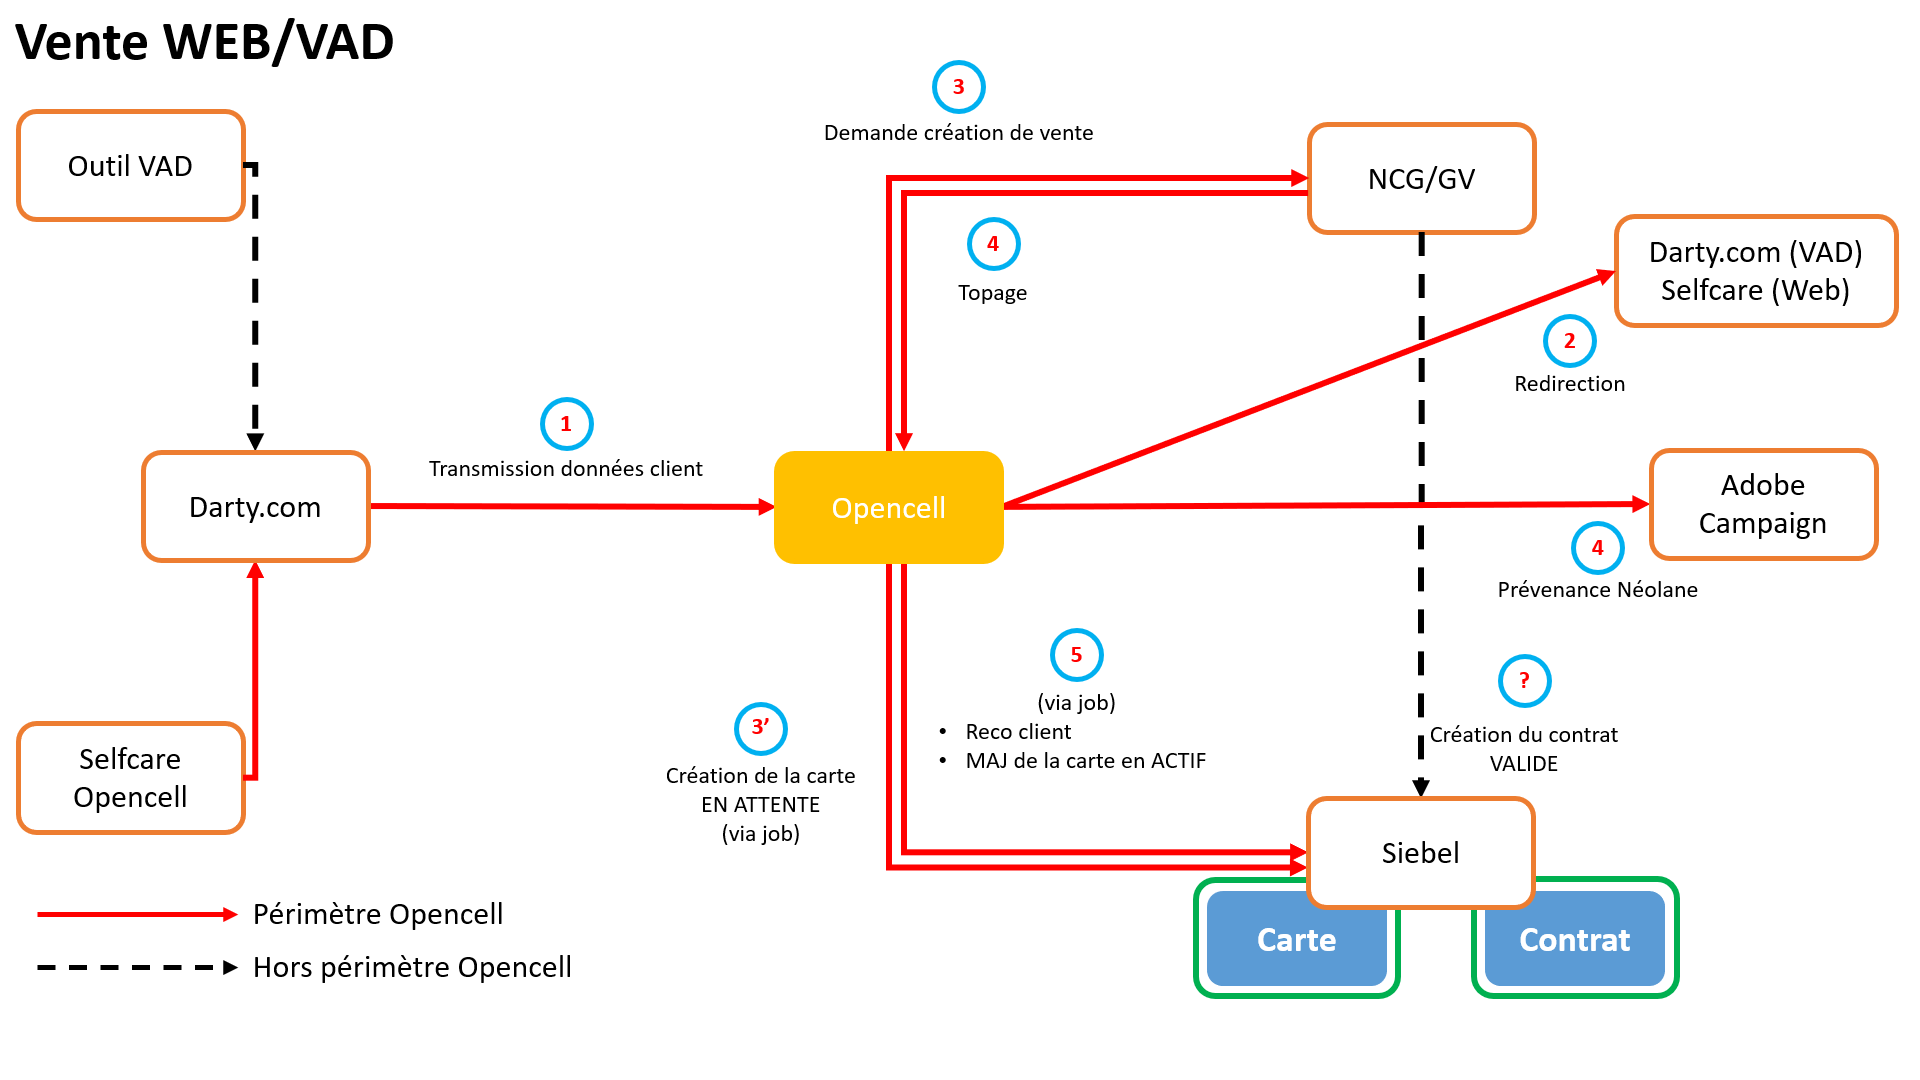
\includegraphics[width=0.8\textwidth]{assets/images/vente_webvad.png}
		\caption{Schéma simplifié des échanges pour une souscription en VAD ou Web}
	\end{figure}
	\vspace{.5cm}
	\begin{figure}[!h]
		\centering
		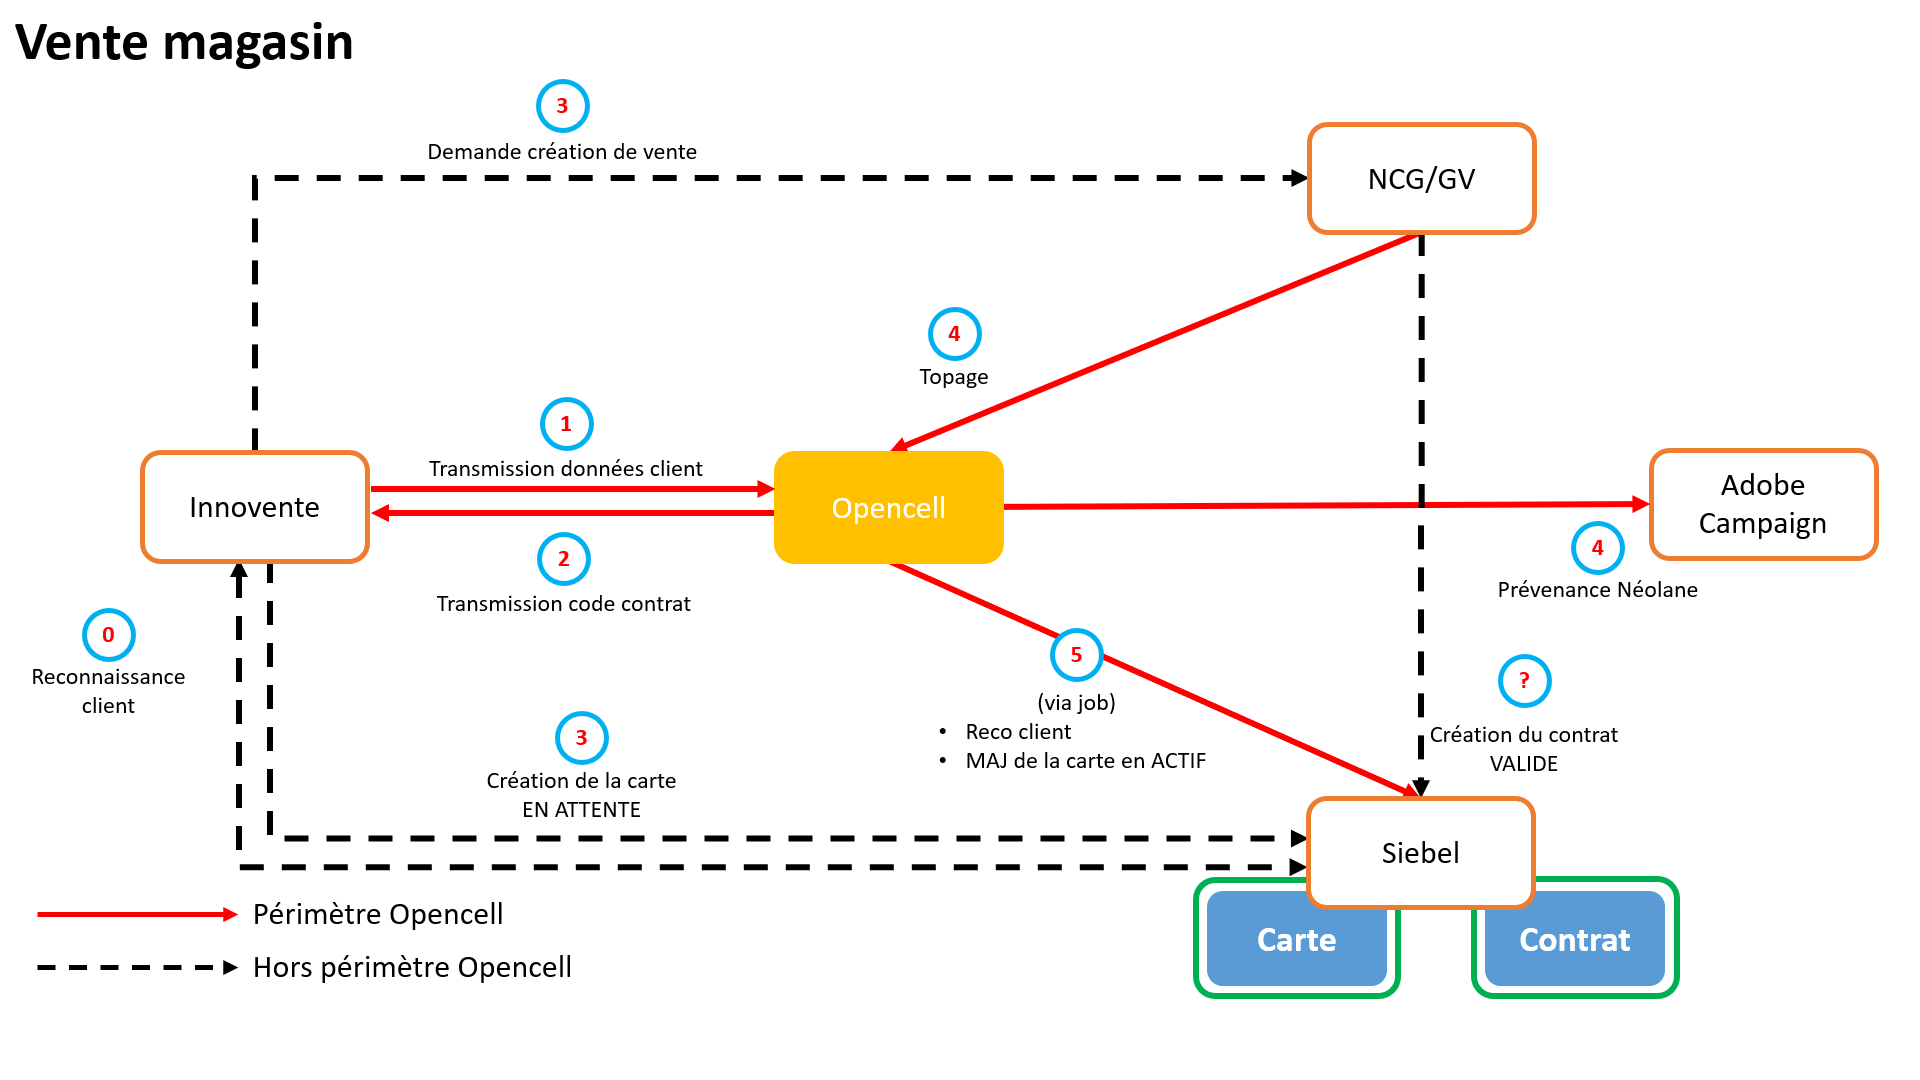
\includegraphics[width=0.8\textwidth]{assets/images/vente_magasin.png}
		\caption{Schéma simplifié des échanges pour une souscription en magasin}
	\end{figure}
	\vspace{.5cm}
	\begin{figure}[!h]
		\centering
		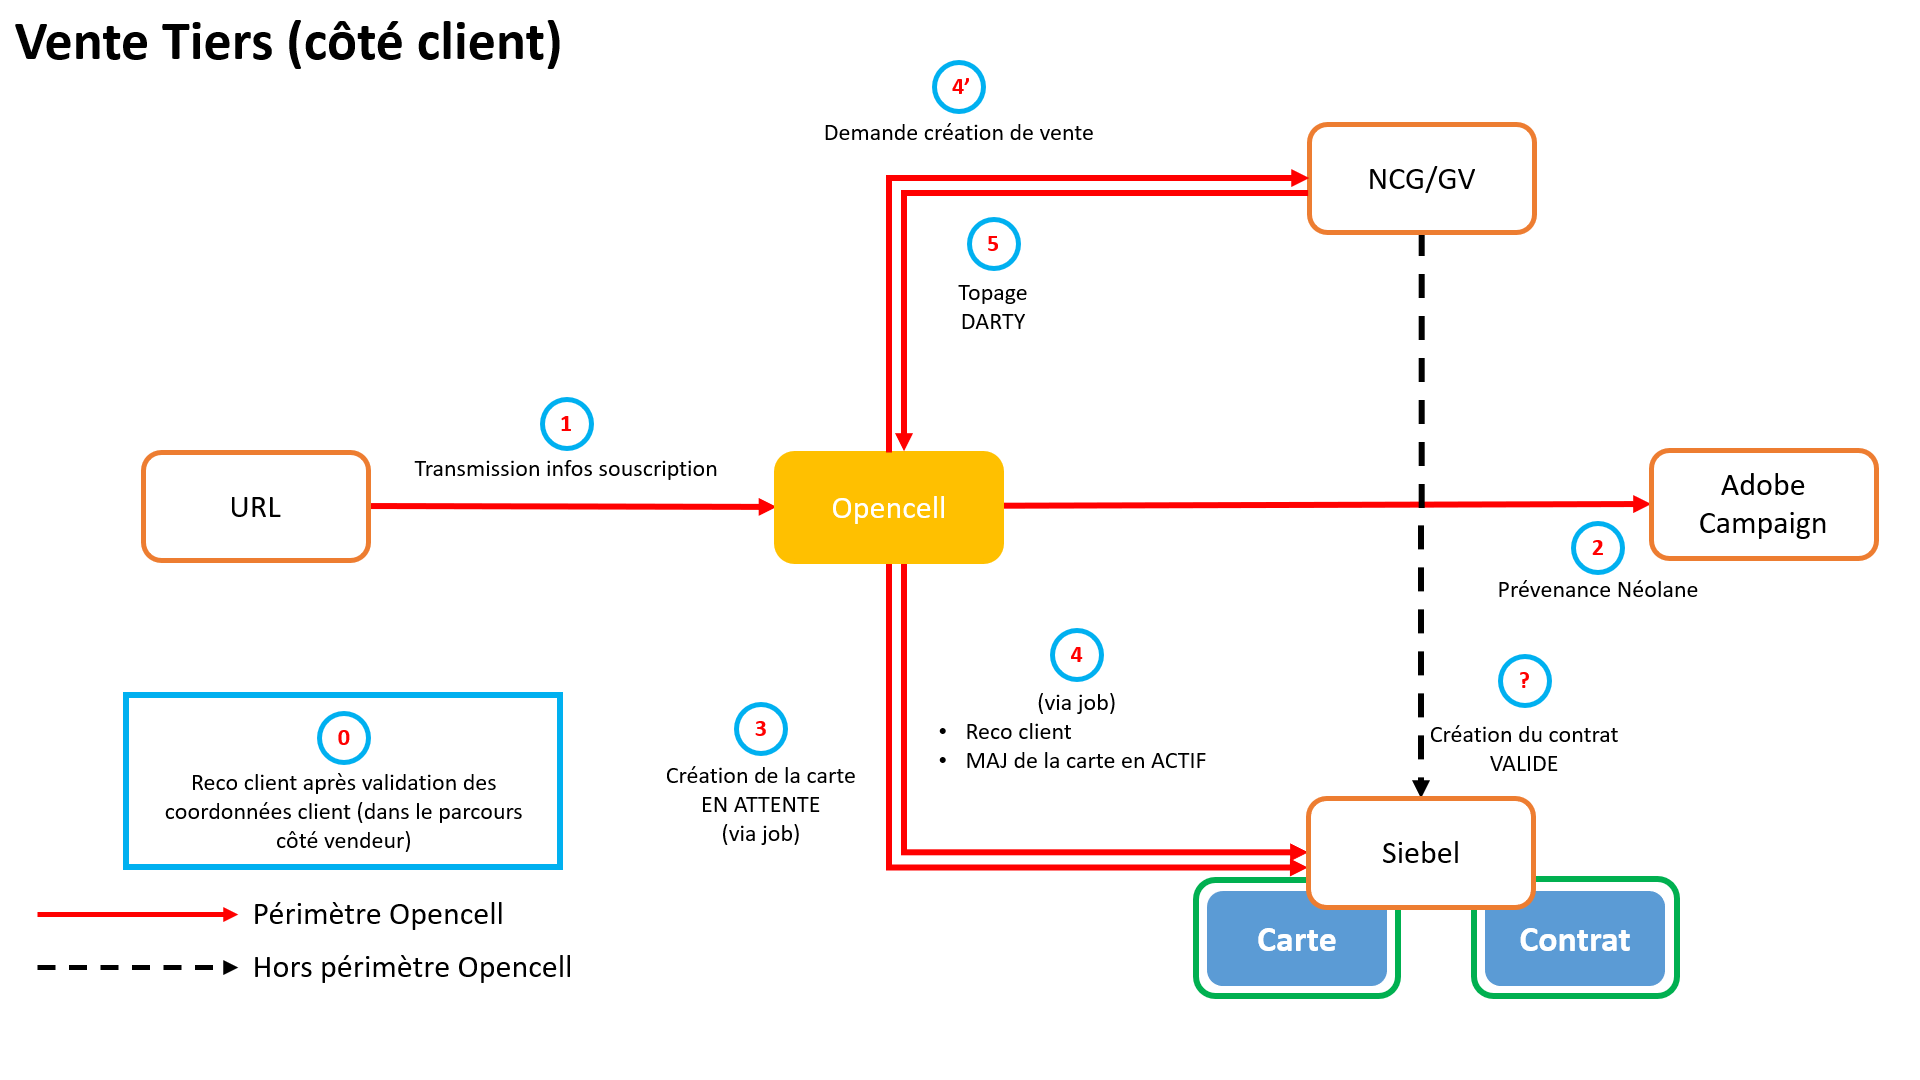
\includegraphics[width=0.8\textwidth]{assets/images/vente_tiers.png}
		\caption{Schéma simplifié des échanges pour une souscription par un tiers}
	\end{figure}

	\newpage
	\subsection{Le Customercare}
	Le Customercare est une application dédiée à l'accompagnement client. Il peut servir entre autres de support technique. Ce service permet d'accéder à toutes les données concernant le client, et permet également la résiliation d'une souscription à tout moment si le client en fait la demande. Il a été développé par Opencell puis repris par CGI.
	\\
	\begin{figure}[!h]
		\centering
		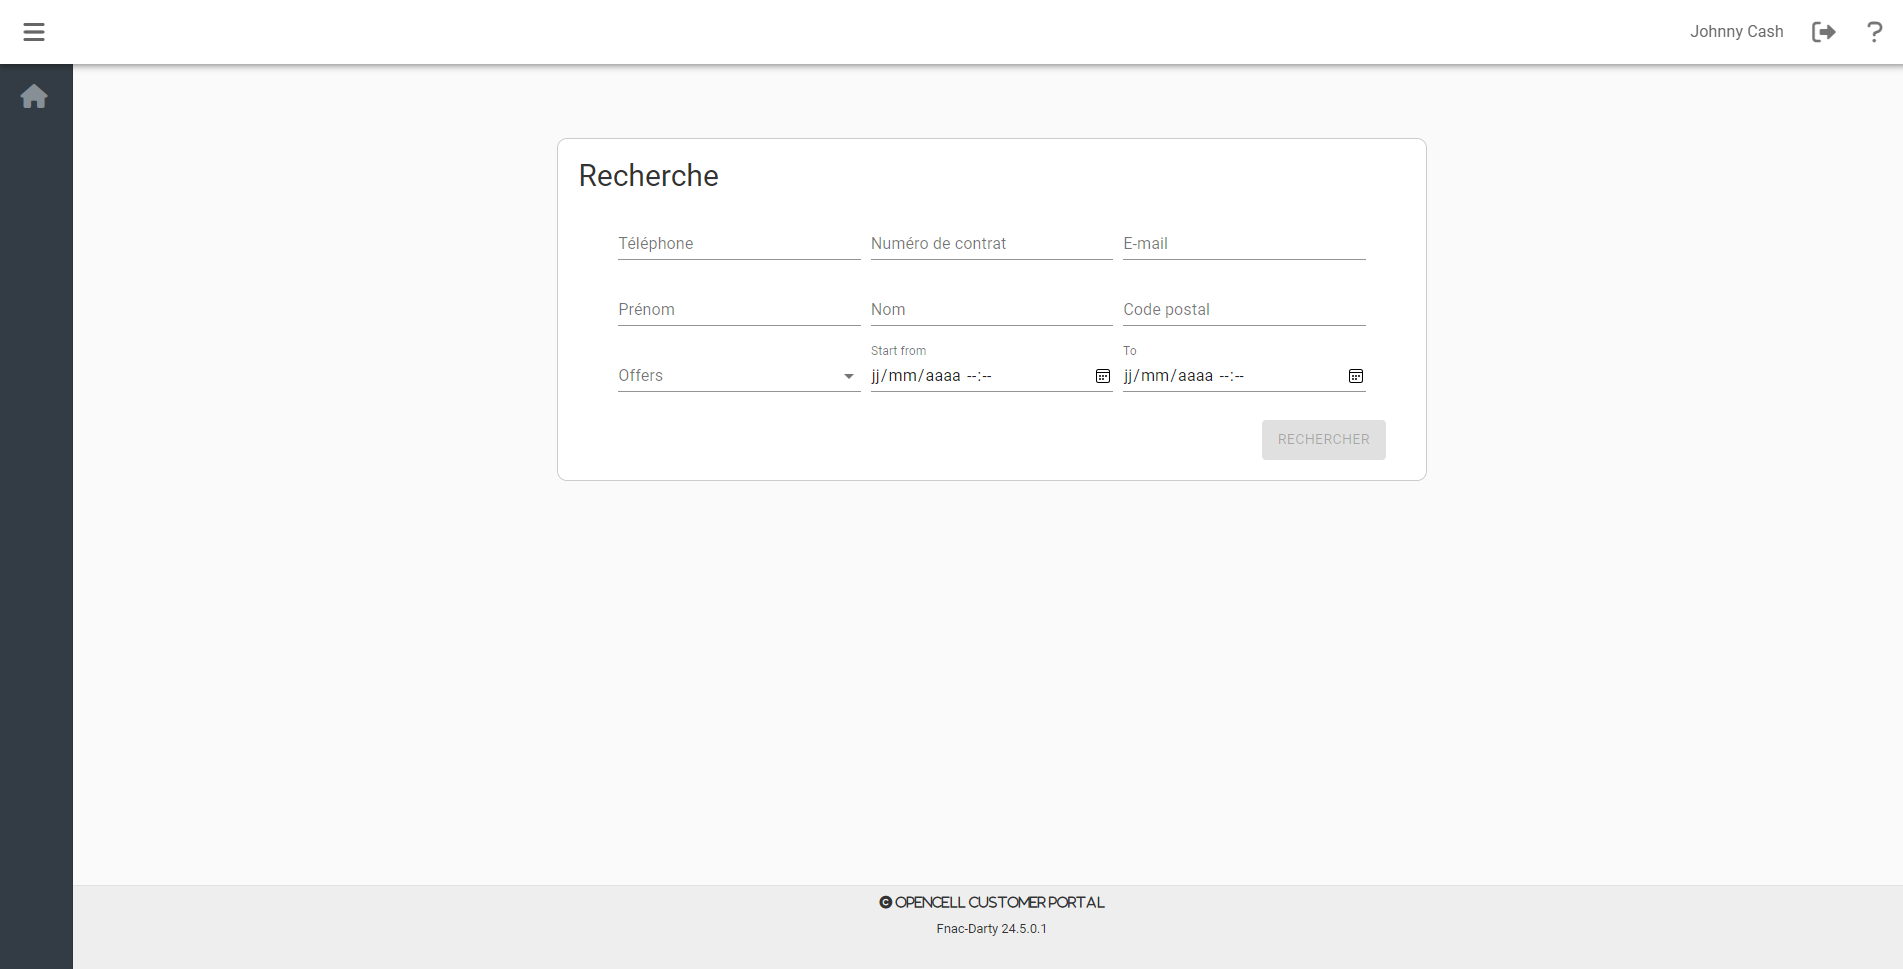
\includegraphics[width=1\textwidth]{assets/images/customercare.png}
		\vspace{-.6cm}
		\caption{Customercare (Service Client)}
	\end{figure}

	\newpage
	\subsection{Le Selfcare}
	Le Selfcare est une application dédiée au client, qui lui permet de gérer/voir ses coordonnées, sa souscription, ses factures et ses documents contractuels (contrat, SEPA\footnote{Single Euro Payments Area (SEPA) est un espace de paiement en euro unifié.}, CGS\footnote{Conditions Générales de Services (CGS) est un ensemble d'informations données par le fournisseur sur les conditions légales d'exécution de ses services.}, etc.). Il permet au client de gérer son abonnement de manière autonome. Tout comme le Customercare, il a été développé par Opencell puis repris par CGI.
	\\\\
	Une rubrique présente les souscriptions associées au compte client pour visualiser les garanties et adhésion de l'individu. Il est possible de consulter ses factures d'achats et le client a la capacité de modifier ses coordonnées. Il peut aussi résilier sa souscription, la modifier ou encore changer le mode de paiement en accédant à celle-ci.

	\begin{figure}[!h]
		\centering
		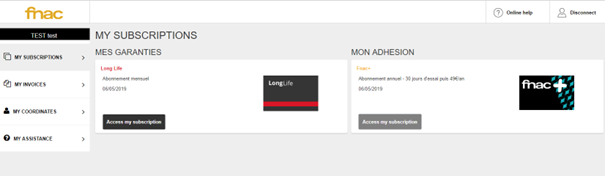
\includegraphics[width=1\textwidth]{assets/images/selfcare.png}
		\vspace{-.6cm}
		\caption{Selfcare (Espace Client)}
	\end{figure}

	\subsection{Extension Opencell}

	Comme son nom l'indique, cette extension d'Opencell permet d'ajouter des fonctionnalités qui ne sont pas présentes dans Opencell, mais dont Fnac/Darty a besoin. Ces fonctionnalités résident dans l'ajout de nouvelles API\footnote{Application Programming Interface (API) est une application par laquelle un logiciel offre des services à d'autres logiciels.}, d'extension des modèles de données (customisation des tables existantes, ajout de nouvelle table, etc.), de créer de nouveau Web Services\footnote{Un Web Service est une technologie qui permet de faire communiquer des applications à distance via internet.}, de créer de nouveaux jobs natifs\footnote{Opencell possède de nombreux jobs qui sont un ensemble de scripts.} ou encore de pouvoir optimiser certaines parties d'Opencell. Cette extension est développée en Java 11.

	\subsection{Bridge}

	Lorsque CGI a repris le projet, l'extension n'existait pas encore et Opencell ne permettait pas de réaliser toutes les demandes de Fnac/Darty. Un Bridge a donc été mis en place pour faciliter les différents traitements et exposer certains Web Services et API. Ce dernier est surtout utilisé pour les parcours Web et VAD ainsi que pour la gestion des exports comptables.

	\subsection{Mock}

	Le mock (ou bouchon Opencell) est une application développée par CGI afin de pouvoir réaliser des tests sur les différents parcours de souscription sur n'importe quel environnements (local, intégration, etc.). Il est mis à disposition de Fnac/Darty pour qu'ils puissent réaliser tout ou partie des tests de leur côté. Cette application, comme l'ensemble des applications front-end, est développée en React.
	\\
	\begin{figure}[!h]
		\centering
		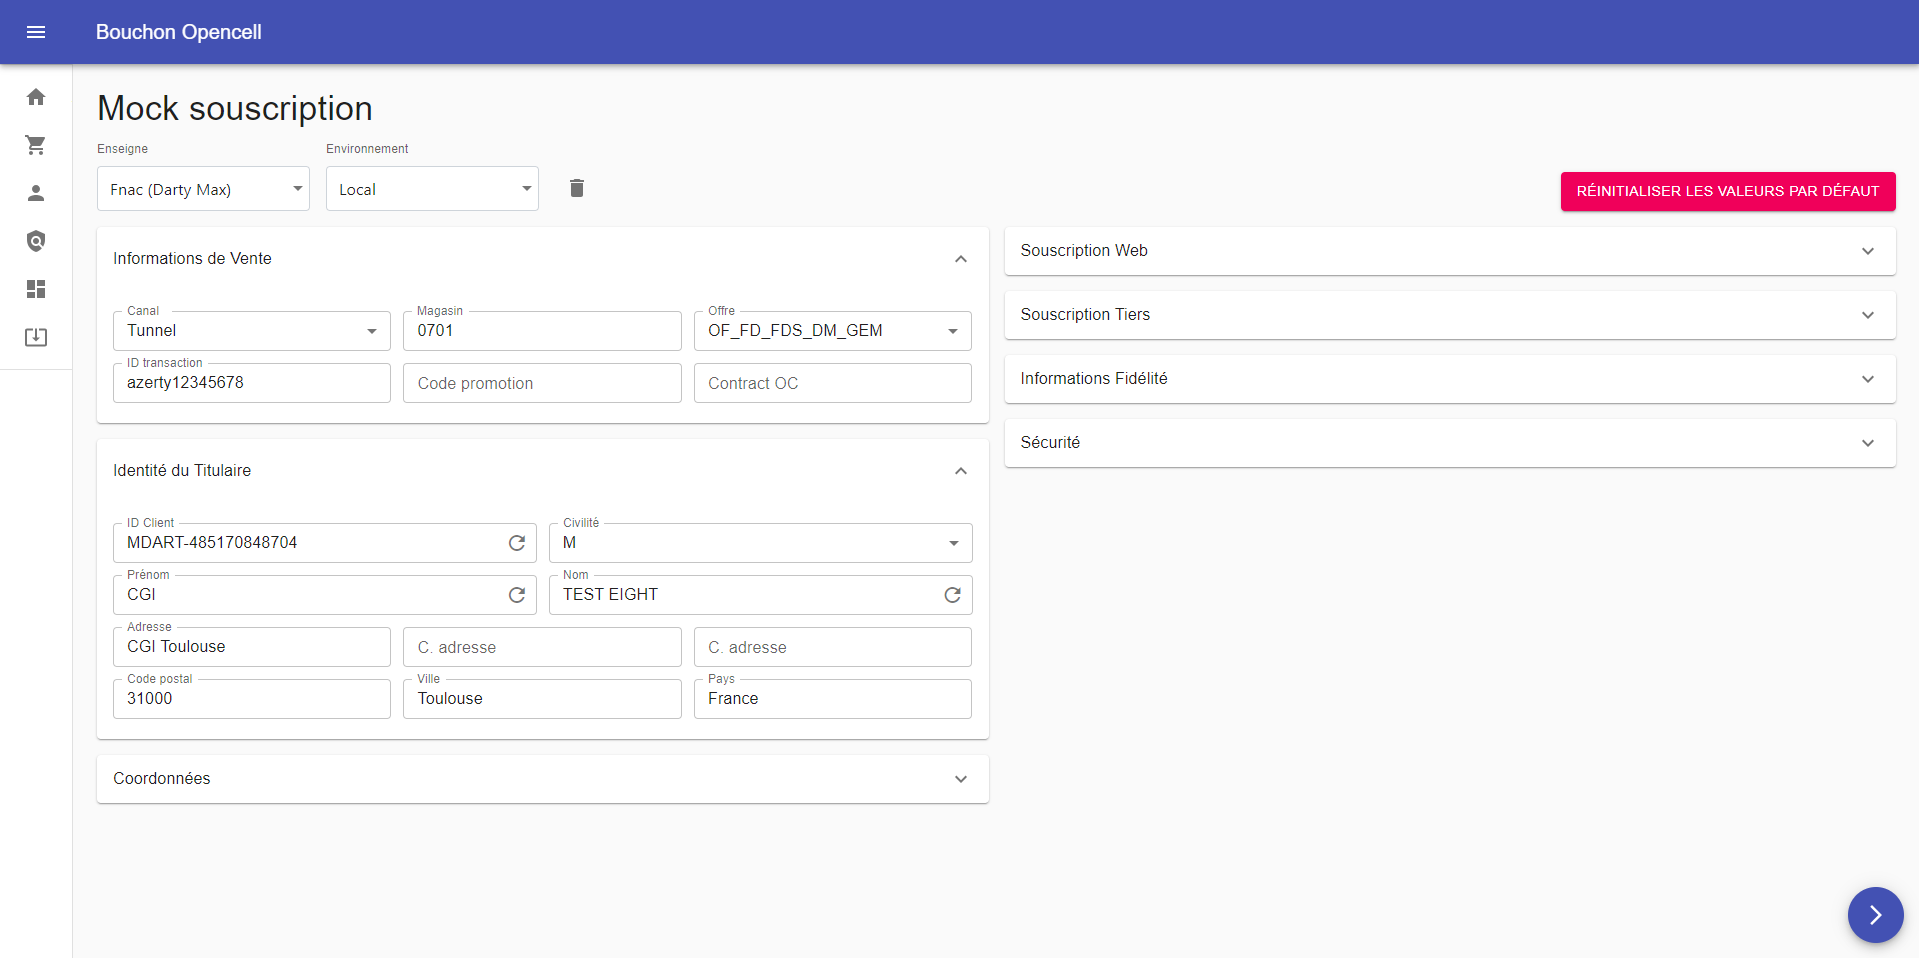
\includegraphics[width=1\textwidth]{assets/images/mock_souscriptions_new.png}
		\vspace{-.6cm}
		\caption{Mock (Bouchon Opencell)}
	\end{figure}
	
	\section{Environnement technique}

	Lors du stage, divers outils ont été utilisés afin de mettre en place une fonctionnalité ou de permettre d'assurer la gestion de projet. La liste de ces outils ainsi qu'une courte présentation de leur utilisation est donnée en \hyperref[sec:outils]{\it{Annexe A}}.
	\\\\
	L'ensemble des applications sont hébergées sur GitLab, qui permet de gérer les différentes versions des applications et revues de code. Les applications sont déployées sur plusieurs environnements\footnote{Détaillés ci-après dans la partie \ref{sec:demarche_tma}} Azure à la charge du client Fnac/Darty. 
	\\\\
	Les différentes applications du projet Fnac/Darty sont développées en Java 11/17 pour le back-end et en React 16/17 pour le front-end. Les applications front-end sont toutes présentes dans le même dépôt GitLab sous la forme d'un monorepo\footnote{Un monorepo est un dépôt de code source qui contient plusieurs applications ou projets dont les bibliothèques/ressources sont partagées.} mis en place via l'outil Nx\footnote{Nx est un outil qui permet de gérer des monorepos en JavaScript/TypeScript.} et dont chaque parcours est une application Nx distincte. Les applications back-end sont elles réparties dans leurs dépôts respectifs.

	\newpage
	\section{Démarche : l'utilisation de la TMA au sein du projet}
	\label{sec:demarche_tma}

	La partie Tierce Maintenance Applicative (TMA) est présente depuis le début du projet, sur l'application Fnac d'abord afin de la maintenir en état en corrigeant les bugs détectés en production puis sur l'ensemble de l'application Fnac/Darty.
	\\\\
	La TMA peut s'utiliser à la fois en mode projet au forfait ou en régie, mais selon des principes légèrement différents comme détaillé ci-dessous. Dans le cadre du projet Fnac/Darty, on peut distinguer les deux utilisations surtout au niveau de la facturation en elle-même.
	\\\\
	Dans le mode au forfait, l'équipe \flqq{} TMA \frqq{} fait en sorte que chaque ticket\footnote{Un ticket peut être considéré ici comme étant un bug ou une évolution.} d'évolution créé au niveau du Jira du client soit chiffré et vendu à un coup unique. Cela se calcule en partie sur le temps estimé pour résoudre/développer le ticket en question. Un ensemble de tickets va être regroupé afin de former un package qui sera livré au client une fois par mois, chaque ticket terminé sera alors vendu et aura une garantie de trois mois si jamais un bug se déclare pour ce ticket là. Cette même garantie est aussi appliquée en mode régie.
	\\\\
	Si le projet TMA se déroule en mode régie, cela veut dire que l'équipe est chez le client, ce n'est pas le cas sur ce projet. Cependant, d'un point de vue de la facturation, l'équipe traite des tickets sans s'engager sur un coût fixe. L'équipe pourra néanmoins \flqq{} macro-chiffrer \frqq{} un ticket afin de donner de la visibilité au client, pour qu'il priorise certains tickets par exemple.
	
	\subsection{La gestion du temps}

	La gestion du temps est abordée de manière différente en TMA par rapport à un développement d'une application en mode Agile où les livraisons du produits sont rythmées par les différents sprints\footnote{Un sprint dans l'utilisation de la méthode Agile représente une phase de développement ayant une durée déterminée, qui a pour objectif de livrer un produit fini.}.
	\\\\
	Dans le cas du projet Fnac/Darty, une Mise En Production (MEP)\footnote{Une mise en production est le fait d'intégrer (déployer) la nouvelle version d'un logiciel dans l'environnement de production.} a lieu environ une fois par mois. À l'occasion de ces différentes livraisons, il peut y avoir des résolutions d'anomalies découvertes depuis la dernière MEP, ou bien des évolutions demandées par le client pour cette nouvelle version. Plusieurs étapes sont nécessaires avant la MEP.

	\begin{enumerate}
		\item Organisation de réunions de préparation au backlog pour délimiter ce qui va être livré.
		\item Développement des nouvelles fonctionnalités et/ou résolutions d'anomalie par les développeurs. Pour cela, la documentation peut être amenée à être mise à jour et des tests d'acceptation de ces fonctionnalités sont réalisés.
		\item Mise en intégration\footnote{L'intégration est un environnement de tests interne côté CGI.} de la nouvelle version de l'application, incluant les tests unitaires et les corrections de bug dans le cas où les tests ont révélé des erreurs.
		\item Mise en recette et pré-production\footnote{La recette et la pré-production sont des environnements de tests côté client.}. Lors de ces phases, le client fait part de son avis, notamment pour savoir s'il y a des bugs ou non, afin de lancer ou non la MEP.
		\item Mise en production.
	\end{enumerate}

	\noindent
	En tant que développeur, il est possible de participer à différentes réunions, qu'il s'agisse de réunions de gestion de projet comme un comité opérationnel\footnote{Le comité opérationnel (comop) est une réunion organisée avec le client afin de faire un suivi du projet sur l'état d'avancement, faire une projection sur ce qui va être réalise et établir un suivi financier.}, ou d'autres réunions avec le client au cours desquelles il s'agit d'interagir sur les différents sujets tel que l'intégration d'une nouvelle fonctionnalité. Cependant, cette activité reste ponctuelle et est moins volumineuse que pour le chef de projet et les experts.
	\\\\
	Pour ma part, je n'ai pas participé à ces réunions. En effet, étant en stage, je n'ai pas eu l'opportunité d'y assister. Ainsi, j'ai pu me concentrer sur des tickets de développement, d'analyse, de documentation, ainsi que sur diverses autres tâches annexes. Une estimation de ma répartition du temps de travail peut être visualisée dans le graphique \ref{fig:temps}.\newline

	\begin{figure}[!h]
		\centering
		\begin{tikzpicture}
			\pie{50/Front-end, 15/Back-end, 10/Tests, 15/Analyse tickets, 5/Documentation, 5/Autre}
		\end{tikzpicture}
		\caption{Estimation du temps de travail tout au long du stage}
		\label{fig:temps}
	\end{figure}

	\noindent
	Cette estimation est basée sur les tickets que j'ai réalisé tout au long du stage. Il important de noter que la part de temps consacrée aux tests est plus importante que ce que le graphique ne laisse paraître. En effet, les tests sont aussi réalisés en parallèle lors du développement.
	\\\\
	Tel qu'on peut le voir sur la figure \ref{fig:temps}, le temps consacré à la partie front-end du projet est bien plus important que celui consacré à la partie back-end. Cela s'explique d'une part par une aisance plus grande dans le développement front-end, mais aussi par le fait qu'il y avait davantage de fonctionnalités, de résolutions de bugs et d'améliorations à réaliser sur la partie front-end du projet.
	\newpage\noindent
	Il est important de noter que la répartition du temps de travail peut varier en fonction des tickets à réaliser. Par exemple, lorsqu'il faut résoudre des anomalies, une grande partie du temps est consacré à trouver la source du problème afin de pouvoir proposer une solution au client\footnote{Cela peut être une simple correction dans le front, comme prévoir une mise en place d'un traitement automatique pouvant rattraper les cas rencontrés.}. Pour cela il faut, selon les cas:
	\\
	\begin{itemize}
		\item[–] Regarder les logs\footnote{En informatique, les logs permettent de garder une trace d'exécution de ce qui se passe en sur les différents serveurs des applications afin de s'assurer du bon fonctionnement.};
		\item[–] Rechercher dans le code de la solution Opencell;
		\item[–] Rechercher dans le code mis en place par CGI (front-end/back-end);
		\item[–] Réaliser des requêtes SQL\footnote{Structured Query Language (SQL) est un language permettant de manipuler des données stockées dans une base de données, ici PostgreSQL.} afin de repérer des cas similaires ou un point commun entre les cas;
		\item[–] Essayer de reproduire l'anomalie sur un autre environnement (le plus souvent en local), cela peut permettre de déterminer si l'anomalie est liée à un environnement spécifique ou non et dans quelle version de l'application elle est apparue.
		\item[–] Utiliser Dynatrace\footnote{Dynatrace est un outil permettant d'assurer la surveillance en temps réel des utilisateurs sur les applications et permet d'analyser plus facilement les causes d'erreur.} pour repérer si possible la trace d'exécution.\\
	\end{itemize}

	\noindent
	Plusieurs points peuvent être nécessaires avant de trouver la cause, il faut donc pour cela être polyvalent, autonome (et parfois créatif) afin de comprendre les différents mécanismes qui ont amené à la création du ticket.

	\subsection{Suivi des travaux et reportings au client}

	Deux environnements Jira sont utilisés dans le cadre de la gestion du projet. Un premier Jira côté client est constamment alimenté afin de pouvoir directement communiquer avec le client et tracer l'avancement des différents tickets. Le second est utilisé en interne, il permet au chef de projet de pouvoir justifier les imputations réalisées au niveau des feuilles de temps des différentes personnes de l'équipe.
	\\\\
	La création d'un ticket peut se faire de plusieurs manières, comme détaillé ci-après.
	\\
	\begin{itemize}
		\item[–] S'il s'agit d'une nouvelle fonctionnalité, le ticket est alors fait par le client.
		\item[–] Un client Fnac/Darty peut appeler le service client et dans certains cas, cela peut amener à la création d'un ticket, notamment si on retrouve une récurrence pour un même type de cas.
		\item[–] Le ticket peut être céé par l'équipe Fnac/Darty lors des tests sur les différents environnements suite par exemple à une nouvelle livraison de l'application.\\
	\end{itemize}

	\noindent
	Certains tickets peuvent demander la réalisation d'un chiffrage par l'équipe CGI afin d'estimer les différents besoins techniques qui y sont rattachés. De façon générale, ce sont les experts qui le réalisent.

	\newpage
	\noindent
	Les tickets sont ensuite priorisés dans le backlog et affectés à une version future de l'application dont la livraison est prévue dans les mois suivants. Une nouvelle version de l'application peut contenir autant de correction d'anomalies que de nouvelles fonctionnalités. Si certaines anomalies se trouvent être urgentes pour le client, une livraison exceptionnelle peut être réalisée en amont des livraisons planifiées.
	\\\\
	L'ensemble des tickets du Jira suivent un workflow\footnote{Un workflow est une suite de tâches qui permettent de réaliser une action.} prédéfini, qui permet de suivre l'avancement de chaque ticket :
	\\
	\begin{itemize}
		\item[–] \textbf{À faire :} le ticket est prêt à être pris en charge;
		\item[–] \textbf{En cours :} le ticket est en cours de développement/analyse par un membre de l'équipe CGI;
		\item[–] \textbf{Dev. bloqué / pause :} le ticket se trouve être en attente d'autres cas pour mieux analyser le ticket ou en attente de réponse de l'éditeur Opencell par exemple;
		\item[–] \textbf{Code review :} Le développement et/ou l'analyse est terminé(e), une fois contrôlé par un autre membre de l'équipe projet, le ticket pourra être livré;
		\item[–] \textbf{Livrée en intégration Darty :} une livraison de la nouvelle version de l'application a été réalisée en interne afin de procéder à des tests avant une livraison officielle au client;
		\item[–] \textbf{Livrée en recette Darty :} le ticket est livré au client, c'est à lui de tester si le ticket est bien conforme à ses attentes;
		\item[–] \textbf{Fermé :} une fois que toutes les étapes précédentes sont réalisées ou que le ticket a été abandonné.
	\end{itemize}

	\newpage

	\begin{figure}[!h]
		\vspace{4cm}
		\centering
		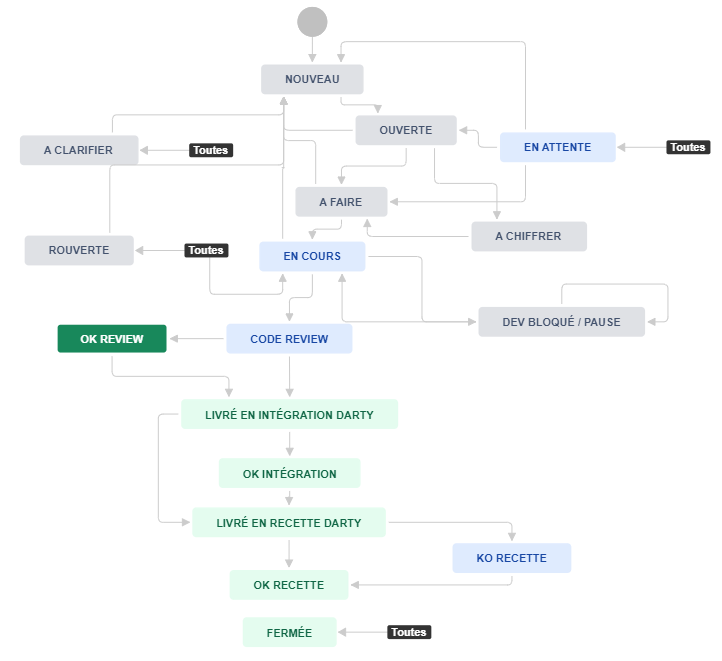
\includegraphics[width=1\textwidth]{assets/images/workflow_jira.png}
		\caption{Workflow des tickets sur le Jira}
	\end{figure}

	\newpage
	\subsection{Agilité au sein de la TMA}

	Lors de la mise en place du projet pour la commercialisation de l'offre Darty Max, l'équipe CGI a utilisé la méthode Agile. Cette dernière est utilisée pour développer des produits ou des services. Cette méthode est devenue populaire, car elle change du fonctionnement classique de la gestion de projet. Elle permet notamment d'apporter plus de valeur aux clients et aux utilisateurs. Cette méthode est aussi appréciée, car elle améliore la satisfaction du travail pour les membres de l'équipe. Par exemple, en Agile, l'équipe de développement doit être auto-organisée et pluridisciplinaire.
	\\\\
	Un des aspects de l'Agilité se trouve être encore aujourd'hui utilisé sur le projet, le Daily meeting.
	\\\\
	Le Daily Meeting, ou simplement Daily, est une réunion quotidienne qui dure une dizaine de minutes. Elle est dirigée pour le projet Fnac/Darty par le chef de projet, qui apporte les connaissances sur l'avancée de l'équipe et s'il y a ou non des blocages. Il permet de définir les sujets du jour à traiter et contrôle le temps de parole pour éviter de s'éterniser sur chaque sujet. Des réunions supplémentaires peuvent bien entendu être planifiées si des sujets ont besoin de plus de discussion, mais ils seront alors traités en dehors du Daily.
	\\\\
	Le Daily meeting se déroule en donnant la parole à tour de rôle aux personnes présentes qui doivent à trois questions :
	\\
	\begin{itemize}
		\item[–] Qu'ai-je fais depuis le dernier Daily ?
		\item[–] Que vais-je faire jusqu'au prochain Daily ?
		\item[–] Quels sont les points de blocage que je rencontre ou que l'équipe rencontre ?\\  
	\end{itemize}

	\newpage
	\section{Travaux réalisés et compétences acquises}

	Durant cette période de stage, j'ai pu participer a de nombreuse tâches, que ce soit du développement pur, de l'analyse et de la résolution d'anomalies, de la documentation, des tests, ou encore des mise à jours de dépendances et de la réécriture de code.

	\subsection{Premiers jours}

	J'ai directement été intégré au projet Fnac/Darty dès mon arrivée. En revanche, j'ai dû commencer par effectuer et valider les différents e-learnings requis pour les nouveaux arrivants à CGI. Ces derniers sont en réalité plusieurs modules de formation en ligne pour apprendre le fonctionnement de CGI, rappeler les règles de sécurité, de vivre ensemble, etc. Ces e-learnings sont obligatoires pour tous les nouveaux arrivants et doivent être validés avant de pouvoir commencer à travailler sur un projet.
	\\\\
	En parallèle des e-learnings, j'ai pu installer les différents outils nécessaires ainsi que l'environnement de développement. Il est composé de trois principaux dépôts Git :
	\\
	\begin{itemize}
		\item[–] \textbf{Apps :} contient le code source des différents parcours de souscription et du mock ainsi que les différentes configurations du projet. C'est avec lui que l'on peut lancer l'application en local.
		\item[–] \textbf{Opencell Extension :} contient la surcouche de l'application Opencell, c'est un overlay Maven\footnote{Un overlay Maven permet d'ajouter des fonctionnalités (développées ici en Java 11) à celles existantes de base dans un logiciel Java (Opencell en l'occurrence).}.
		\item[–] \textbf{Bridge :} cette application reprend les fonctionnalités demandées par Fnac/Darty, mais qui ne s'intègrent pas dans Opencell et qui ne peuvent pas être ajoutées dans Opencell Extension.\\
	\end{itemize}

	\noindent
	Une fois les e-learnings terminés et le projet installé sur mon poste, j'ai pu commencer la prise en main du projet. Tout d'abord, j'ai été affecté à de petites fonctionnalités ou de petits correctifs de bugs. Cela m'a permis de me familiariser avec le code et les différentes technologies utilisées sur le projet. 
	\\\\
	Une de ces fonctionnalités se trouve être l'ajout d'un parseur d'URL\footnote{Uniform Resource Locator (URL) est l'adresse d'un site ou d'une page internet.} sur le Mock afin de faciliter la séparation des arguments passés en paramètre de l'URL. C'est une simple fonctionnalité de QoL\footnote{Quality of Life (QoL) est une fonctionnalité qui n'apporte pas de nouvelles fonctionnalités à l'utilisateur, mais qui améliore l'expérience utilisateur.} pour les testeurs qui peuvent ainsi plus facilement décrypter les arguments passés en paramètre de l'URL.
	\\\\
	En effet, les souscriptions via le parcours Tiers envoient par mail une URL encryptée au client pour qu'il puisse continuer la suite du parcours par lui-même (renseigner ses moyens de paiements et signer le contrat). Le Mock permet de décrypter (ou d'encrypter) cette URL, permettant aux développeurs de vérifier que les informations envoyées sont correctes et que le parcours se déroule bien.
	\newpage\noindent
	Or pour déchiffrer l'URL, il fallait manuellement copier-coller les arguments de l'URL dans chacune des zone de texte et l'affichage des données obtenues n'était pas très lisible (voir \hyperref[sec:mock_before]{Annexe C}). Par conséquent, mon équipe à juger bon de me confier cette première tâche. 
	\\\\
	Pour répondre à ce besoin, j'ai choisi tout simplement d'ajouter une nouvelle zone de saisie pour l'URL encryptée et de récupérer les arguments depuis cette dernière. Il est important de noter que la zone d'arguments de l'URL commencent par un \flqq{} \texttt{?} \frqq{} et que chaque argument est déclaré selon le format \flqq{} \texttt{clef=valeur} \frqq{} et séparé par un \flqq{} \texttt{\&} \frqq{}. J'ai donc simplement séparé les chaque argument et préremplis leurs zone de texte respective (voir \hyperref[sec:mock_after]{Annexe D}).
	
	\begin{figure}[!h]
		\begin{minted}[bgcolor=cverbbg]{text}
https://fnacdarty.com/index?data=<encrypted>&iv=<token>
		\end{minted}
		\vspace{-.8cm}
		\caption{Exemple d'URL encryptée}
	\end{figure}
	
	\noindent
	Afin de rendre les données obtenues plus lisible, j'ai fait en sorte que le JSON\footnote{JavaScript Object Notation (JSON) est un format de données textuelles permettant de représenter des objets JavaScript.} décrypté soit affiché de manière structurée et colorée pour pouvoir différencier les champs et leurs valeurs. J'ai également ajouté un bouton pour copier les résultats directement dans le presse-papier. Ces nouvelles fonctionnalités ont été très appréciées par les utilisateurs qui ont pu gagner du temps lors de leurs tests.
	\\\\
	Enfin, j'ai pu livrer ces nouvelles fonctionnalités directement en production via le serveur FTP\footnote{File Transfer Protocol (FTP) est un protocole de communication dédié à l'échange de fichiers sur un réseau TCP/IP.} de CGI. Cela m'a permis de voir directement l'impact de mon travail et des responsabilités qui m'étaient confiées. Cette mise en jambe m'a permis de me familiariser avec le process de développement, de test et de déploiement de nouvelle fonctionnalité sur le projet.
	
	\newpage
	\subsection{Premiers mois}

	Suite à cela et pendant environs les trois premiers mois de mon stage la charge de travail s'est graduellement intensifié et j'ai pu participer à de nombreuses tâches. J'ai notamment pu travailler sur la mise en place de nouvelles fonctionnalités avec l'anonymisation des contrats résiliés et quelques optimisations.

	\subsubsection{Anonymisation des contrats résiliés}

	% AnonymisationFullJob

	Tout d'abord, Fnac/Darty avait des attentes spécifiques concernant la purge des données que la mécanique native d'Opencell ne pouvait pas/plus satisfaire. La fonctionnalité d'anonymisation des données clients d'Opencell ne permettait que leur suppression, tandis que le client souhaitait conserver une trace des souscriptions résiliées tout en respectant les législations européennes, notamment le RGPD\footnote{Règlement Général sur la Protection des Données (RGPD) est un règlement de l'Union Européenne qui encadre le traitement des données personnelles des individus.}. De plus, la fonctionnalité existante n'était plus à jour et ne couvrait plus l'ensemble des données clients ajoutées via l'extension Opencell, ce qui posait problème lors de l'anonymisation.
	\\\\
	Pour satisfaire ce besoin, le client souhaitait que la nouvelle mécanique d'anonymisation des contrats résiliés puisse répondre aux exigences suivantes :
	\\
	\begin{itemize}
		\item[–] Pouvoir anonymiser les données clients avec une fréquence configurable et une durée de rétention des données avant anonymisation exprimée en année;
		\item[–] Prendre en compte les impacts dans le Selfcare;
		\item[–] Prendre en compte les impacts dans le Customercare.
	\end{itemize}
	\vspace{.5cm}

	\noindent
	Pour répondre à ces besoins, j'ai dû travailler sur la création d'un nouveau job Opencell. En effet, Opencell possède un ensemble de jobs natifs qui permettent de réaliser des tâches spécifiques de manières automatique et/ou planifiées. Ces jobs sont présents dans l'application et l'ajout d'un nouveau job est impossible sans passer par l'extension. La façon \flqq{} officielle \frqq{} d'Opencell pour remplir des fonctions similaires à un job serait de créer un script\footnote{Les scripts Opencell sont de petites fonctions écrite en Java qui peuvent être créés à la demande pour réaliser des tâches spécifiques et exécutés de manière automatique et/ou régulière, sans avoir à modifier le code source d'Opencell.}, mais ces derniers peuvent présenter des problèmes de performances et de scalabilité (détaillé ci-après dans \hyperref[s:amelioration_performances]{\it{Amélioration des performances}}).
	\\\\
	J'ai donc été amené à implémenter un nouveau job en utilisant l'extension d'Opencell : \cverb|AnonymizeFullJob|. Ce job permet d'anonymiser le contrat résilié et toute sa hiérarchie\footnote{Dans Opencell, les données clients sont organisées selon une hiérarchie précise.} si nécessaire. En effet, Fnac/Darty avait des attentes spécifiques concernant la hiérarchie des données clients. Si tous les contrats d'un utilisateur sont résiliés, alors il faut anonymiser l'utilisateur, son compte et son compte client etc. jusqu'à la souscription. Cela permet de conserver une trace des souscriptions résiliées tout en respectant les législations européennes.
	
	\newpage
	\noindent
	En pratique, les données clients sont organisées selon la hiérarchie suivante : un \cverb|Customer|\footnote{Représente un utilisateur de l'application.} (Cu) possède un ou plusieurs \cverb|CustomerAccount|\footnote{Représente le compte global d'un client qui inclut toutes les informations de l'utilisateur.} (CA) possède un unique \cverb|BillingAccount|\footnote{Sert de lien entre le CA et le UA en centralisant les informations de facturation, assurant que toutes les transactions des UAs sour un CA soient correctement enregistrées et facturées.} (BA) qui possède un unique \cverb|UserAccount|\footnote{Désigne le compte individuel d'un utilisateur spécifique au sein d'un CA, permettant à cet utilisateur d'accéder aux services et fonctionnalités en fonction de ses droits.} (UA) qui lui peux posséder une ou plusieurs\footnote{Uniquement si l'utilisateur a changé d'offre via un downgrade ou un upgrade.} \cverb|Subscription|\footnote{Les souscriptions sont les contrats signés par les utilisateurs pour bénéficier des services proposés par Fnac/Darty.}.
	\\\\
	Par conséquent il a été nécessaire de s'assurer que toutes les souscriptions avaient été résiliées depuis $X$ années avant de pouvoir anonymiser son UA, puis en faire de même pour le BA et le CA. Là encore, il a fallu s'assurer que les données ajoutées via l'extension Opencell soient bien prises en compte lors de l'anonymisation, avec notamment la suppression\footnote{Fnac/Darty ne souhaitait pas anonymiser ces données dans la mesure ou elles n'apportent pas de réelles plus-value.} des données d'historisation sur les changements apportés aux contrats désormais anonymisés.
	\\\\
	Pour anonymiser les données, Fnac/Darty souhaitait que chaque champ permettant d'identifier l'utilisateur soient remplacées par la chaîne de caractères \cverb|ANONYM_uuid_id| où l'UUID\footnote{Un UUID (Universal Unique Identifier) est un identifiant unique de 128 bits, utilisé pour identifier de manière unique des informations dans des systèmes distribués. Il est souvent représenté sous forme de chaîne de 32 caractères hexadécimaux.} est un identifiant unique généré pour chaque utilisateur anonymisé.
	\\\\
	Enfin, dans la mesure où les données anonymisées ne sont plus supprimées par Opencell, il a fallu modifier le Selfcare et le Customercare pour que les différents appels à l'API ne retournent plus les données anonymisées et qu'il ne soit plus possible de les afficher.

	\newpage
	\subsubsection{Amélioration des performances}
	\label{s:amelioration_performances}

	Plus tard lors de mon stage, j'ai pu travailler sur la réécriture d'un script Opencell en job natif. En effet, Fnac/Darty avait remarqué que le script \cverb|AnonymizePaymentMethodScript| n'anonymisait jamais les données lorsque la volumétrie de ces dernières était trop importante.
	\\\\
	En réalité, les scripts sont exécutés par Opencell de manière séquentielle, c'est-à-dire que chaque donnée que le script traite est traitée l'une après l'autre. Cela ne pose en général pas de problème pour de petits volumes de données ou pour de petites opérations, mais ce n'était pas le cas ici.	
	\\\\
	Il était donc nécessaire de réécrire ce script en job natif pour résoudre ce problème, car les jobs natifs peuvent être écris de manière à pouvoir traiter les données en parallèle. Ainsi, de la même manière que pour le job mentionné précédemment, j'ai dû créer un nouveau job Opencell \cverb|AnonymizePaymentMethodJob| via l'extension. 
	
	\begin{figure}[!h]
		\centering
		
\includegraphics[width=1\textwidth]{assets/images/abo_3845_before.png}
		\vspace{-.6cm}
		\caption{Les résultats avant réécriture du script}
		\label{fig:abo_3845_before}
	\end{figure}

	\begin{figure}[!h]
		\centering
		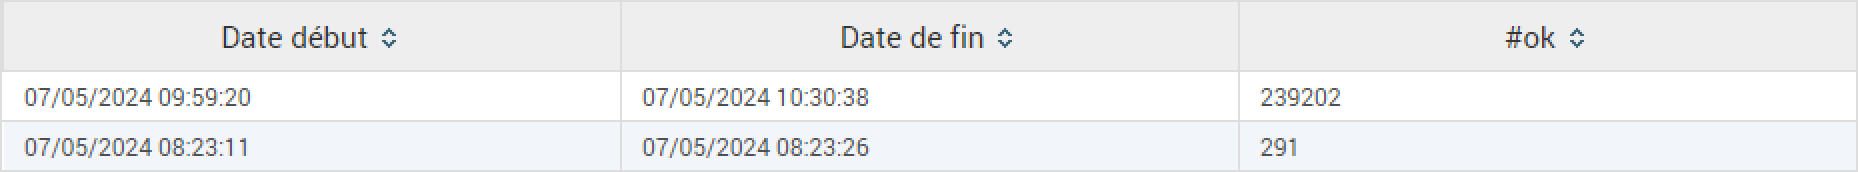
\includegraphics[width=1\textwidth]{assets/images/abo_3845_after.png}
		\vspace{-.6cm}
		\caption{Les résultats après réécriture du script}
		\label{fig:abo_3845_after}
	\end{figure}

	\noindent
	Avant la réécriture, le script s'exécutait pendant plusieurs heures (voir \ref{fig:abo_3845_before}) avant d'être interrompu par Opencell. Après la réécriture du script en job natif, l'exécution de ce dernier ne prenait plus que quelques minutes (voir \ref{fig:abo_3845_after}) avec 10 000 cas supplémentaires, ce qui représente un gain de performance considérable.
	
	\newpage
	\subsection{Fin du stage} 
	
	Les deux derniers mois de mon stage ont été plus léger en terme de nouvelle fonctionnalité et correction d'anomalies. Ce qui a permis à mon équipe et moi-même de pouvoir nous concentrer sur de l'optimisation et de la réécriture de code. J'ai notamment pu travailler sur la mise à jour des dépendances, la mise en place de Redux Toolkit et l'extraction des types de l'API.

	\subsubsection{Typage et extraction des types de l'API}	
	
	Dans la mesure où les premières plateformes de souscriptions ont été développées par Fnac/Darty en JavaScript, une partie de ces dernières n'ont pas été typées correctement ou ne l'ont pas été du tout lors de la migration vers TypeScript\footnote{TypeScript est un sur-ensemble de JavaScript ajoutant des fonctionnalités de typage statique qui améliorent la robustesse et la maintenabilité du code.}. 
	\\\\
	Cela cause plusieurs problèmes lors du développement, mais aussi lors de l'utilisation des différents parcours. En effet, le typage incorrect ou inexistant peut entraîner une obfuscation du code, une augmentation du temps de développement et de nombreux bugs. 
	\\\\
	Cela est dû, d'une part par la présence de nombreux types \flqq{} any \frqq{} qui rendent difficile la compréhension du code. Ces derniers se propagent dès qu'on les utilises (voir \ref{fig:type_any}),	ce qui amène des valeurs de tout type à circuler sans contrôle par TypeScript, augmentant le risque d'erreurs à l'exécution et rendant le code plus difficile à relire/maintenir\footnote{L'utilisation du type \flqq{} any \frqq{} a pour effet de masquer les erreurs potentielles et d'empêcher les développeurs de bénéficier pleinement des avantages offerts par TypeScript, tels que l'autocomplétion et la vérification des types à la compilation.} (et cela rend aussi l'utilisation de TypeScript caduque). D'autre part, les différents parcours n'ont pas tous été typé de la même manière, ce qui peut amener à des erreurs ou des incompréhensions lors de l'utilisation de ces derniers à de mauvais endroits. Enfin, l'API d'Opencell suivant une certaine structure, il est possible d'unifier le typage des réponses de l'API pour en faire profiter l'ensemble des applications front.
	\\\\
	C'est pourquoi tout au long de mon stage, j'ai été amené à typer (ou re-typer) certaines parties du code. Cette tâche a impliqué non seulement la conversion manuelle des fichiers existants, la mise à jour de TypeScript pour répondre aux besoins spécifique, mais aussi l'utilisation d'outils automatisés pour faciliter le processus. Par exemple, j'ai pu utiliser le plugin Maven \cverb|cz.habarta.typescript-generator| pour générer les interfaces et enums TypeScript à partir des DTO\footnote{Le Data Transfer Object (DTO) est un objet qui transporte des données entre les différentes couches de l'application.} Java d'Opencell et de son extension. 
	\\\\
	Hélas, je n'ai pas réussi à automatiser cette génération pour que les types utilisés côté TypeScript soient toujours synchronisés avec les structures de données définies en Java. Le plugin Maven ne réussissait pas à générer un fichier TypeScript correct et devait être corrigé manuellement. L'automatisation d'un tel processus pourrait à terme réduire ainsi les risques d'incohérences et de bugs liés aux changements de schéma.

\newpage
\begin{figure}[!h]
\begin{minted}[bgcolor=cverbbg, linenos]{typescript}
function majAny(value: any) {
  return value.toUpperCase();
}

function majString(value: string) {
  return value.toUpperCase();
}

// Meh, compile mais test1 sera de type `any` car TypeScript ne peut
// pas déterminer le type de retour de `any`.toUpperCase()
const test1 = majAny('hello');

// KO, le code suivant compile mais cause une erreur à l'exécution
// car Number.toUpperCase() n'existe pas en JavaScript :
// >> Uncaught SyntaxError: Invalid or unexpected token
const test2 = majAny(42);

// OK, compile et test3 sera de type `string` 
// (car la méthode String.toUpperCase retourne une String)
const test3 = majString('hello');

// OK, Ne compile pas car majString attend une chaîne de caractères
// Aucune erreur à l'exécution car TypeScript empêche la compilation
// >> Type 'number' is not assignable to type 'string'.
const test4 = majString(42);
\end{minted}
\vspace{-.8cm}
\caption{Exemple des problèmes liés à l'utilisation du type \flqq{} any \frqq{}}
\label{fig:type_any}
\end{figure}

	\noindent
	Pour pouvoir centraliser les types et enums\footnote{Un enum (pour énumération) est un type de données qui permet de définir un ensemble de constantes nommées.} entre les différentes applications du monorepo, j'ai créé deux répertoires du même nom dans le répertoire \flqq{} shared \frqq{} à la racine du monorepo. Cette organisation facilite la réutilisation des types et des enums dans différentes parties du projet, améliorant ainsi la cohérence et la maintenabilité du code. Le partage de ces définitions communes permet également d'éviter la duplication de code et les erreurs qui peuvent en résulter, tout en garantissant que toutes les applications utilisent les mêmes types, ce qui simplifie le développement et le débogage.

	\newpage
	\subsubsection{Mise à jours des dépendances}
	% [refactor] ABO-000 : Update dependencies 
	% https://gitlab.com/fnacdarty/fdps/dev/teams/services/opencell/opencell-apps/-/merge_requests/1167

	Le projet ayant été repris par CGI en 2019, certaines dépendances utilisées n'ont jamais été mises à jour depuis. Par conséquent, certaines dépendances pouvaient présenter des failles de sécurité, des bugs ou des problèmes de performance. Il était donc nécessaire de les mettre à jour pour ses raisons.
	\\\\
	De plus, les dépendances dépendent parfois les unes des autres, il était nécessaire de les mettre à jour dans un ordre précis pour éviter tout problème de compatibilité. Par exemple, la mise à jour de TypeScript a entraînée la mise à jour d'ESLint\footnote{ESLint est un outil de linting pour JavaScript et TypeScript qui permet de détecter les erreurs de syntaxe et de style dans le code source.} et celle de NodeJS\footnote{NodeJS est un environnement d'exécution JavaScript côté serveur basé sur le moteur JavaScript V8 de Google Chrome.} à conduit à la mise à jour de Webpack\footnote{Webpack est un outil de build qui permet de transformer, regrouper et empaqueter les fichiers JavaScript et CSS.} et de Nx.

	\paragraph{TypeScript}
	% Maj TS 3.9 -> 5.4

	Au fur et à mesure de mes avancées sur diverses fonctionnalités, j'ai pu constater que certaines fonctionnalités de TypeScript dont j'avais l'habitude manquait pour répondre à certains de mes besoins. Par exemple, dans la version 3.9 utilisée alors sur le projet, il n'était pas possible d'utiliser les \flqq{} templates strings \frqq{} pour les types. Or, cette fonctionnalité est très utile pour définir des types de manière dynamique. Par exemple, pour définir un type de fichier, il est possible d'utiliser un \flqq{} template string \frqq{} pour définir le nom du fichier et son extension de manière dynamique. Cela permet de s'assurer que le nom du fichier est bien une chaîne de caractères et que l'extension est bien valide. Voici un exemple de typage utilisant les \flqq{} templates strings \frqq{} :
	
	\begin{figure}[!h]
	\begin{minted}[bgcolor=cverbbg, breaklines]{typescript}
type extension = "jpg" | "png" | "gif";   // union types
type filename = `${string}.${extension}`; // template strings

const file1: filename = "a.jpg";  // OK
const file2: filename = "a.gif";  // OK

const file3: filename = "a";      // KO, l'extension est manquante
const file4: filename = "a.jpeg"; // KO, l'extension n'est pas valide
const file5: filename = "42.png"; // KO, le nom du fichier n'est pas une chaîne de caractères
	\end{minted}
	\vspace{-.8cm}
	\caption{Exemple de typage utilisant les \flqq{} templates strings \frqq{}}
	\end{figure}

	\noindent
	TypeScript est très conciliant lors des mises à jour, il est donc possible de le mettre à jour sans avoir à modifier le code existant ni de risquer de créer des régressions\footnote{Une régression est un bug qui apparaît dans une nouvelle version d'un logiciel et qui n'était pas présent dans la version précédente.}. Cela permet de bénéficier des dernières fonctionnalités et améliorations apportées par les nouvelles versions aisément tout en assurant une rétrocompatibilité avec les anciennes versions.
	\\\\
	Enfin, j'ai pu en profiter pour mettre en commun les configurations TypeScript des différentes applications du monorepo. Cela a permis de supprimer les parties redondantes et de standardiser les règles de compilation pour l'ensemble des applications.
	
	\paragraph{Webpack et Nx}
	% NodeJS 16 -> 18 => Webpack 4 -> 5 => Nx 10 -> 18

	La migration de Webpack 4 à 5 s'est avérée nécessaire suite au passage à NodeJS 18. En effet, la version LTS\footnote{Long Term Support (LTS) est une version d'un logiciel qui bénéficie d'un support à long terme, c'est-à-dire que des correctifs de sécurité et des mises à jour de maintenance sont publiés pendant une période prolongée.} précédente de NodeJS n'était plus supportée et présentait une faille de sécurité avec les certificats SSL\footnote{Secure Sockets Layer (SSL) est un protocole de sécurisation des échanges sur internet.}, corrigée dans sa version LTS suivante, NodeJS 18. Mais dès lors, Webpack 4 n'était plus compatible et il a fallu le mettre à jour pour garantir la compatibilité avec la nouvelle version de NodeJS.
	\\\\
	Les applications des différents parcours étant gérées par Nx, qui utilise Webpack 4, il a également été nécessaire de le mettre à jour. Pour cela, je suis directement passé de la version 10 à la version 18 de Nx. Cette tâche à nécessité quelques modifications sur les différents fichiers de configurations de Nx, mais ces dernières se sont avérées fortement utiles pour la suite du projet. En effet, la version 18 de Nx apporte de nombreuses améliorations et corrections de bugs, ce qui a permis de gagner en performance et en stabilité.
	\\\\
	Pour revenir sur Webpack, la mise à jour de la version 4 à 5 a apportée beaucoup de changement dans la façon dont sont gérées les dépendances et les fichiers de configurations. Webpack 5 change du tout au tout et cela a été un vrai défis de migrer sur cette nouvelle version sans causer de régressions. 
	\\\\
	Cela a nécessité de revoir l'ensemble des fichiers de configurations Webpack pour les adapter. J'ai dû également comprendre pleinement le fonctionnement de Webpack et de ses différentes parties (les loaders, les plugins, les entrées, les sorties, etc.). Enfin, j'ai pu comprendre comment fonctionne un bundler\footnote{Un bundler est un outil qui permet de regrouper et de transformer les fichiers sources d'une application en un seul fichier de sortie.} et comment il permet d'assembler et de regrouper les différents fichiers sources en un seul fichier de sortie.
	\\\\
	Pour simplifier la gestion du projet, j'ai également unifié les configurations Webpack des différentes applications du monorepo. Ne gardant que les parties spécifiques à chaque application, j'ai pu supprimer les parties redondantes et standardiser les règles de compilation pour l'ensemble des applications.
	\\\\
	La mise à jour vers Webpack 5 a également permis de réduire le temps de compilation des applications, car Webpack 5 est plus rapide que Webpack 4. C'est un gain de temps non-négligeable pour les développeurs qui peuvent ainsi voir les changements apportés au code plus rapidement et plus facilement.

	\newpage
	\paragraph{Material UI 5 et React 17}
	% souhait d'utiliser MUI 5 mais requiert React 17 => Mise à jour de React mais impossible d'avoir 2 versions de React dans le même projet, donc switch vers PNPM pour gérer les dépendances.

	Suite à l'ajout d'une nouvelle fonctionnalité sur le Mock, il a été décidé de mettre à jour Material UI\footnote{Material UI est une bibliothèque de composants React basée sur les principes du Material Design de Google.} (MUI) vers sa version 5. En effet, la version 4 de Material UI n'était plus mis-à-jour depuis fin 2021 et la volonté d'utiliser certaines fonctionnalités de la version 5 ont poussés à la migration. Or, la version 5 de Material UI requiert à minima React 17 pour fonctionner. Impliquant la nécessité de mettre à jour React 16 vers la version 17 pour répondre aux exigences de compatibilité de MUI 5.
	\\\\
	Cependant, une difficulté importante est apparue : il est impossible d'avoir deux versions différentes de React dans le même projet en raison des conflits potentiels et des incompatibilités entre les différentes versions de bibliothèques utilisant React. Ce problème est lié à la gestion des dépendances par NPM\footnote{Node Package Manager (NPM) est le gestionnaire de librairies par défaut de NodeJS.} et de l'utilisation de Nx pour gérer la mise en commun des dépendances entre les différentes applications du monorepo. En effet, les composants React partagés entre différentes applications se retrouvent alors avec deux versions possible de React, causant ce problème.
	\\\\
	Ce problème a conduit à une réévaluation de la gestion des dépendances du projet et même de la structure du projet en monorepo pour trouver une solution. Après plusieurs recherches et discussions, il a été décidé de garder la structure du monorepo pour économiser du temps et de l'énergie, mais aussi de garder ces dépendances partagées. 
	\\\\
	Ainsi, pour garder la structure de monorepo, il a été décidé de changer le manager de dépendances pour PNPM\footnote{PNPM est un autre manager de librairies de NodeJS.}. Ce dernier permet, via l'utilisation de workspaces\footnote{Un workspace PNPM est un ensemble de packages qui partagent les mêmes dépendances et qui sont installés dans le même répertoire node\_modules.}, de partager certaines dépendances uniquement entre certaines applications/modules du monorepo (voir \ref{fig:directory_tree}). De plus, PNPM permet de gérer les dépendances de manière plus efficace que NPM, en les stockant dans un cache global et en les liant symboliquement dans les différents workspaces, ce qui permet de réduire l'espace disque utilisé et le temps de téléchargement des dépendances.

	\newpage
	\vspace*{3cm}

	\begin{figure}[!h]
		\begin{multicols}{2}
		\dirtree{%
			.1 /.
			.2 apps/.
			.3 mock/.
			.3 tiers/.
			.3 \dots.
			.2 libs/.
			.3 ui/.
			.3 \dots.
			.2 node\_modules/.
			.3 axios@0.28.
			.3 react@16.
			.3 mui@4.
			.3 \dots.
			.2 package.json.
			.2 package-lock.yaml.
			.2 \dots.
		}
		\columnbreak
		\dirtree{%
			.1 /.
			.2 apps/.
			.3 mock/.
			.4 node\_modules/.
			.5 react@17.
			.5 mui@5.
			.5 \dots.
			.4 \dots.
			.3 tiers/.
			.4 node\_modules/.
			.5 react@16.
			.5 mui@4.
			.5 \dots.
			.4 \dots.
			.3 \dots.
			.2 libs/.
			.3 ui/.
			.4 node\_modules/.
			.5 react@*.
			.5 \dots.
			.4 \dots.
			.3 \dots.
			.2 node\_modules/.
			.3 axios@0.28.
			.3 \dots.
			.2 package.json.
			.2 pnpm-lock.yaml.
			.2 pnpm-workspace.yaml.
			.2 \dots.
		}
		\end{multicols}
	\label{fig:directory_tree}
	\caption{Structure du projet avant (à gauche) et après (à droite) le passage à PNPM}
	\end{figure}

	\newpage
	\subsubsection{Implémentation de Redux Toolkit}

	Chaque parcours requérant de garder en mémoire un grand nombre d'informations (aussi appelées \flqq{} états \frqq{}) à travers les différentes pages, l'utilisation de Redux\footnote{Redux est une bibliothèque JavaScript open-source pour gérer les différents états d'une application.} s'est avérée nécessaire pour garantir la cohérence des données et la synchronisation des différents composants. Cependant, l'intégration de Redux peut parfois être lourde et complexe, nécessitant une configuration détaillée avec de nombreuse étapes, comme la création d'actions\footnote{Une action est un objet qui décrit un changement de l'état de l'application.}, de reducers\footnote{Un reducer est une fonction qui prend en entrée l'état actuel de l'application et une action, et retourne un nouvel état.} et de stores\footnote{Le store est un objet qui contient l'état de l'application et permet d'accéder à cet état et de le modifier.}. Ce qui peut rapidement rendre le code verbeux et difficile à maintenir.
	\\\\
	Redux Toolkit est conçu pour répondre à ces défis en simplifiant et en rationalisant l'utilisation de Redux. Il offre des outils comme \cverb|createSlice| qui combine les actions et les reducers en une seule entité, et \cverb|createAsyncThunk|, qui facilite la gestion des effets secondaires asynchrones\footnote{Les effets secondaires asynchrones sont des opérations qui ne peuvent pas être exécutées immédiatement et qui nécessitent un certain temps pour être complétées, comme les appels réseau ou les requêtes à une base de données.}. Ces abstractions réduisent considérablement la quantité de code standard, ce qui rend le processus de développement plus rapide, plus intuitif et moins sujet aux erreurs. De plus, Redux Toolkit intègre des pratiques optimales, comme l'immutabilité\footnote{L'immutabilité est le concept selon lequel les objets ne peuvent pas être modifiés une fois qu'ils ont été créés.} automatique, et configure par défaut des outils essentiels comme Redux DevTools\footnote{Redux DevTools est une extension qui permet de visualiser et de déboguer l'état de l'application Redux directement dans le navigateur.}, offrant ainsi un environnement de développement plus robuste.
	\\\\
	Par conséquent, l'adoption de Redux Toolkit au sein des applications front a permis et permettra d'optimiser le flux de travail en réduisant la complexité et en améliorant la maintenabilité du code. Ainsi les applications pourront être développées plus rapidement et le risque d'erreurs sera minimisé grâce à une gestion des états plus claire et plus efficace. En somme, Redux Toolkit offre un moyen moderne et puissant de tirer le meilleur parti de Redux tout en simplifiant les processus nécessaires à son utilisation.

	\newpage
	\subsubsection{Assurer la rétrocompatibilité}

	% Appli tierce de Fnac/Darty utilisant les parcours front via Chrome 79

	Les différents parcours pouvant être utilisés par des applications tierces\footnote{Ces applications sont développées au sein de Fnac/Darty et CGI n'a pas la main dessus.}, il a été nécessaire de garantir la rétrocompatibilité des applications après ces mise à jours. En effet, certaines de ces applications tierces utilisent des versions de navigateur très anciennes (tel que Chrome 79, sorti fin 2019) et qui ne supportent pas les dernières nouveautés de JavaScript (voir \ref{fig:can_i_use_chaining_operator}). Redux Toolkit, par exemple, utilise des fonctionnalités de JavaScript qui n'existait pas encore à l'époque de Chrome 79. Il était donc nécessaire de s'assurer que les applications tierces puissent continuer à utiliser les parcours sans problème, quel que soit le navigateur utilisé.
	
	\begin{figure}[!h]
		\centering
		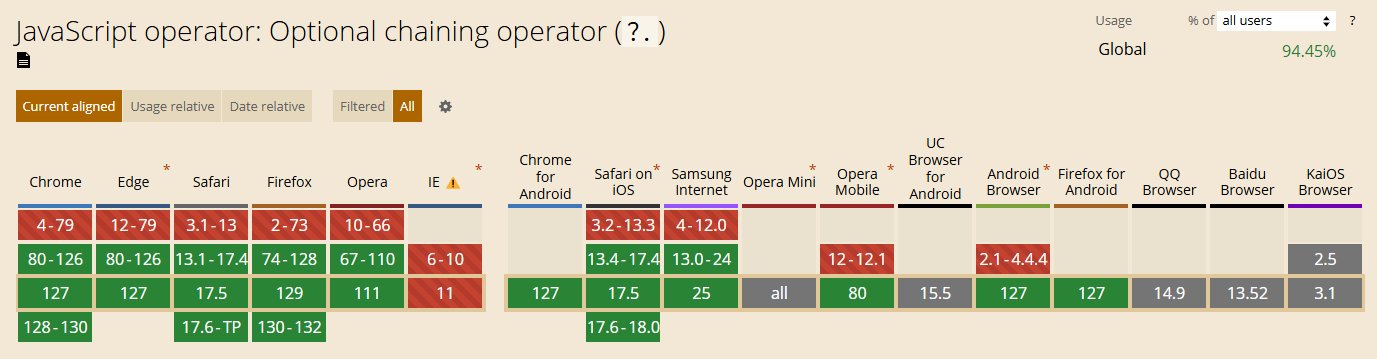
\includegraphics[width=1\textwidth]{assets/images/can_i_use_chaining_operator.png}
		\vspace{-.6cm}
		\caption{Compatibilité de l'opérateur de chaînage optionnel sur \href{https://caniuse.com/mdn-javascript_operators_optional_chaining}{\textit{Can I Use}}}
		\label{fig:can_i_use_chaining_operator}
	\end{figure}
	
	Pour cela, le projet utilisait déjà Babel\footnote{Babel est un outil de compilation qui permet de transformer le code JavaScript moderne en code JavaScript compatible avec les anciennes versions de navigateurs.} pour transpiler\footnote{À la différence de la compilation, la transpilation consiste en la conversion de code d'un langage de programmation vers un autre langage de haut niveau, sans créer de code machine exécutable directement.} le code JavaScript moderne en code compatible avec des navigateurs plus anciens. J'ai donc pu ajouter les plugins nécessaires et réparer les différentes librairies non-supportées manuellement pour garantir la compatibilité des applications avec d'anciennes versions de navigateurs.

	\begin{figure}[!h]
	\begin{minted}[bgcolor=cverbbg, breaklines]{typescript}
//--- TypeScript 5.4
const obj: Record<string, string | undefined> = { a: 'Hello World!' };

// L'opérateur de chaînage optionnel (?.) permet de vérifier
// si une propriété existe avant de l'accéder pour éviter les erreurs
const out = obj.a?.toUpperCase(); // 'HELLO WORLD' ou undefined

//--- JavaScript ES10
const obj = { a: 'Hello World' };
const out = obj.a === null || obj.a === undefined 
  ? undefined 
  : obj.a.toUpperCase();
	\end{minted}
	\vspace{-.8cm}
	\caption{Exemple de code utilisant une fonctionnalité non-supportée par Chrome 79}
	\label{fig:optional_chaining}
	\end{figure}
	
	\newpage\noindent
	Pour résumé, les différents parcours sont compilés selon le schéma \ref{fig:compilation_front}, dans lequel TypeScript transpile le code source en JavaScript ES14\footnote{ECMAScript 14 est la version du standard ECMAScript sortie en 2023, qui est la spécification standardisée de JavaScript}. Ensuite, Babel transpile les fonctionnalités non-supportées en ajoutant des polyfills\footnote{Un polyfill est un morceau de code (ou un plugin) qui intègre des fonctionnalités modernes/manquantes à des navigateurs qui ne les supportent pas nativement.} et/ou via des transformations de code (voir \ref{fig:optional_chaining}) pour obtenir du JavaScript ES10 et garantir la compatibilité avec les anciennes versions de navigateurs.
	
	\begin{figure}[!h]
		\centering
		\begin{tikzpicture}[
			node distance=2cm,
			box/.style={rectangle, draw, text centered, minimum height=1cm, minimum width=2.5cm},
			arrow/.style={-Stealth, thick}
		]

		% Nodes
		\node[box] (ts) {TypeScript 5.4};
		\node[box, right=of ts] (js) {JavaScript ES14};
		\node[box, right=of js] (babel) {JavaScript ES10};

		% Arrows
		\draw[arrow] (ts) -- (js) node[midway, below=.6cm] {};
		\draw[arrow] (js) -- (babel) node[midway, below=.6cm] {};

		\end{tikzpicture}
		\vspace{-.3cm}
		\caption{Étapes de "compilation" des applications front}
		\label{fig:compilation_front}
	\end{figure}
	
	\newpage
	\subsubsection{Unification des linters}
	\label{sec:linters}

	Le projet étant basé sur un monorepo, chaque application possède ses propres fichiers de configuration parmi lesquels ce trouve celui d'ESLint. Cela peut s'avérer pratique dans le cas de spécificités propres à une application, mais cela peut aussi être source de problèmes. En effet, chaque application ayant été créée à des moments différents, les configurations ESLint se sont retrouvées à être très différentes d'une application à l'autre, ce qui peut être source de confusion et d'erreurs à la fois pour les développeurs et pour l'IDE\footnote{Un Environnement de Développement Intégré (IDE) est un logiciel qui regroupe des outils de développement logiciel en un seul environnement graphique.} qui ne sait plus quelle configuration utiliser en cas de conflit.
	\\\\
	Pour répondre à ce problème, j'ai pu unifier les configurations ESLint des différentes applications du monorepo dans un seul fichier partagé à la racine du monorepo. Cela a permis de supprimer grand nombre de règles superflues (qui sont déjà présentes dans les règles ESLint par défaut) et de standardiser les règles de style et de syntaxe à respecter pour l'ensemble des applications (certaines applications enlevaient les points-virgules à la fin des lignes, d'autres les ajoutaient, etc.)
	\\\\
	Enfin, j'ai pu intégrer les IDEs des développeurs (voir \hyperref[sec:outils]{\it{Annexe A}}) pour qu'ils utilisent cette configuration partagée. Cela a permis de garantir que peu importe l'application sur laquelle ils travaillent, les développeurs respectent les mêmes règles de style et de syntaxe à l'aide des règles définies dans les fichiers d'EditorConfig\footnote{EditorConfig est un fichier de configuration qui permet de définir et de maintenir des styles de codage cohérents entre différents éditeurs de texte et IDE.} et d'ESLint.
	\\\\
	Une fois les configurations unifiées, j'ai pu lancer ESLint sur l'ensemble des applications du monorepo pour détecter les erreurs de style et de syntaxe. Cela a permis de remonter un grand nombre d'erreurs :

	\begin{figure}[!h]
		\centering
		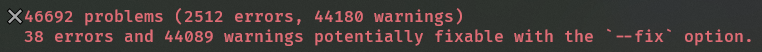
\includegraphics[width=1\textwidth]{assets/images/lint_errors.png}
		\vspace{-.6cm}
		\caption{Erreurs remontées après l'unification sur toutes les applications}
	\end{figure}

	\noindent
	Dans la mesure où la résolution de toutes les erreurs remontées par ESLint n'était pas envisageable, car elle aurait pu être une source de régression et aurait demandée un temps considérable, l'idée de mettre en place un pipeline d'analyse de code m'a été proposée afin de résoudre ces erreurs au fur et à mesure des nouvelles fonctionnalités développées.
	\\\\
	Un pipeline est un ensemble de tâches automatisées exécutées manuellement ou automatiquement selon un paramétrage prédéfini pour répondre aux besoins du CI/CD\footnote{Continuous Integration/Continuous Deployment (CI/CD) est une pratique de développement logiciel qui permet d'automatiser l'intégration du code source dans un référentiel partagé et de le déployer automatiquement dans un (ou plusieurs) environnement.}. Dans le cas présent, l'idée était de modifier le pipeline pour qu'il exécute ESLint uniquement sur les fichiers modifiés par les Merge Requests\footnote{Une Merge Request est une demande de fusion de code source entre deux branches de code source, aussi appelées Pull Request (PR) sur GitHub} (MR) pour éviter de surcharger les MRs avec des fichiers dont la modification ne repose pas sur le but de la MR.
	\\\\
	Par conséquent, j'ai ajouté une étape d'analyse dans le fichier \flqq{} \cverb|.gitlab-ci.yml| \frqq{} (voir \hyperref[sec:ci-cd_gitlab]{\it{Annexe E}}) du projet. Cette étape est exécutée à chaque fois qu'une MR est ouverte et que des commits\footnote{Un commit est une opération qui enregistre les modifications apportées à un fichier ou un ensemble de fichiers dans un dépôt Git.} sont ajoutés à cette dernière. Concrètement, l'étape d'analyse récupère les fichiers modifiés par la MR, en faisant une différence entre la branche visée par la MR et les modifications apportées par cette dernière. Puis,
  elle exécute ESLint uniquement sur ces fichiers. Si ESLint rencontre des erreurs, la MR est annotée avec ces dernières, mais cela ne bloque pas la fusion de la MR (pour éviter de bloquer le travail des autres membres de l'équipe si l'erreur remontée 
	n'est pas bloquante).
	\\
	
	\begin{figure}[!h]
		\centering
		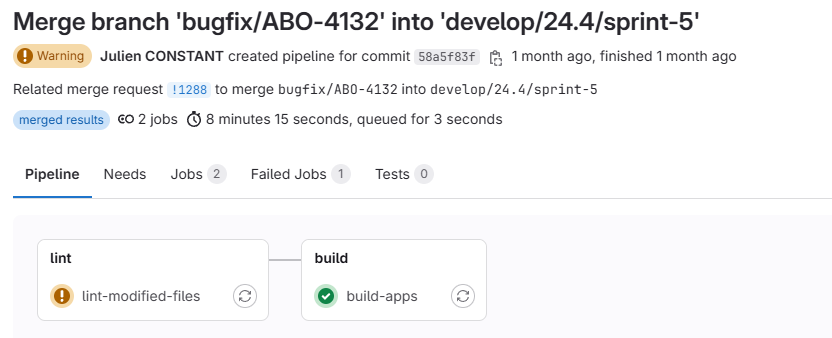
\includegraphics[width=1\textwidth]{assets/images/lint_pipeline.png}
		\vspace{-.6cm}
		\caption{Aperçu du pipeline d'analyse du code}
	\end{figure}

	\newpage
	\subsubsection{Parrallélisation de la compilation des différentes applications front-end}
	
	Suite à la mise à jour des dépendances, j'ai pu constater que le temps de compilation de chaque application avait diminué d'environ 30\%. Mais ce changement ne se reflétait pas sur le pipeline de compilation des applications front-end. En effet, le pipeline compilait les applications une par une, ce qui prenait beaucoup de temps et de ressources, parfois pendant plusieurs dizaines de minutes. Il était donc nécessaire de paralléliser la compilation des applications pour réduire le temps de compilation global.
	\\\\
	Pour se faire j'ai pu utiliser les fonctionnalités de Nx qui permettent de paralléliser les tâches de compilation. J'ai donc modifié le pipeline (voir \hyperref[sec:ci-cd_gitlab]{Annexe E}) de compilation des applications front-end pour qu'il compile les applications en parallèle. Cela a permis de réduire le temps de compilation global à seulement quelques minutes et ainsi de libérer des ressources pour les autres tâches du pipeline GitLab.
	\\

	\begin{figure}[!h]
		\centering
		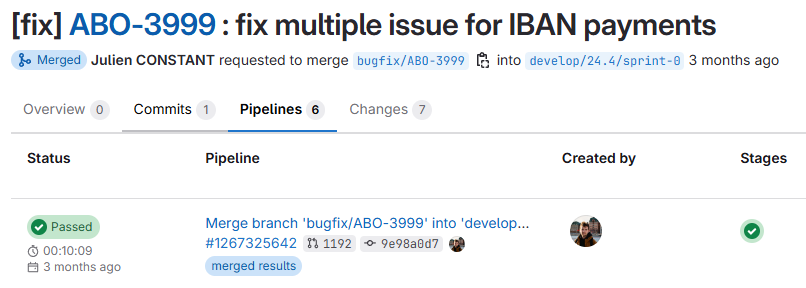
\includegraphics[width=1\textwidth]{assets/images/build_pipeline_before.png}
		\vspace{-.6cm}
		\caption{Temps total du CI/CD avant la parallélisation}
	\end{figure}

	\begin{figure}[!h]
		\centering
		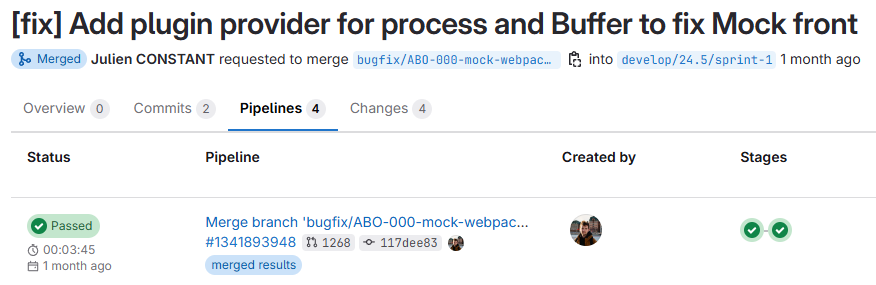
\includegraphics[width=1\textwidth]{assets/images/build_pipeline_after.png}
		\vspace{-.6cm}
		\caption{Temps total du CI/CD après la parallélisation}
	\end{figure}
	
	\chapter{Bilan}
	
	Pour terminer, ce stage de fin d'études chez CGI m'a permis de découvrir davantage le monde de l'entreprise et de mettre en pratique les connaissances acquises durant mes études au sein d'un projet concret et d'une équipe expérimentée. J'ai pu travailler sur un projet de grande envergure pour un client de renom, Fnac/Darty, et j'ai pu contribuer à l'amélioration de la qualité du code et des performances des applications front-end du projet.
	\\\\
	Malgré le fait que les changements apportés par mes différentes missions n'étaient pas toujours visibles directement par le client, j'ai pu constater que mes contributions ont eu un impact positif sur le projet et sur l'équipe. J'ai pu apporter des solutions innovantes et efficaces aux problèmes rencontrés. J'ai également pu travailler en autonomie sur des tâches complexes et prendre des décisions importantes pour le projet. J'ai aussi eu la possibilité de travailler en collaboration avec les autres membres de l'équipe, pour partager mes connaissances et apprendre des autres.
	\\\\
	J'ai pu découvrir de nouvelles technologies et de nouveaux outils, comme Webpack 5 et Nx pour ensuite les mettre en pratique dans un projet réel. J'ai également pu approfondir mes connaissances en TypeScript et en React, qui sont des technologies très utilisées dans le monde du développement web. J'ai également pu découvrir la méthodologie Agile et les pratiques de développement en entreprise, comme les revus de code, les sprints, etc. J'ai pu m'intégrer rapidement dans l'équipe et faire part de mes idées et de mes propositions pour améliorer le projet. Aussi, j'ai pu m'adapter aux différentes situations et contraintes du projet pour trouver des solutions efficaces et adaptées. 
	\\\\
	Pour finir, ce stage m'a permis de développer mes compétences techniques et mes compétences relationnelles, et de redécouvrir le monde de l'entreprise et le monde du travail en général. J'ai pu découvrir le fonctionnement d'une entreprise de services du numérique (ESN) et les différents métiers du développement web. J'ai pu également découvrir le monde du e-commerce et les enjeux liés à la vente en ligne. En somme, ce stage a été une expérience très enrichissante et formatrice pour moi et je suis très heureux d'avoir pu y participer.

	\begin{flushleft}
		\nocite{*}
		\addcontentsline{toc}{chapter}{Bibliographie}
		\setlength\bibitemsep{0.5cm}
		\printbibliography{}
	\end{flushleft}

	\appendix
	\chapter*{Annexes}
	\addcontentsline{toc}{chapter}{Annexes}
	\renewcommand{\thesection}{\Alph{section}}

	\section{Présentation des différents outils utilisés}
	\label{sec:outils}

	\begin{itemize}
		\item[–] \textbf{Confluence :} Confluence est un outil de type wiki, utilisé comme logiciel de travail collaboratif. L'équipe s'en sert pour partager des informations qui concernent le projet comme des modes opératoires.
		\vspace{0.5cm}
		\item[–] \textbf{Dynatrace :} Dynatrace est un outil de surveillance des performances des applications, utilisé pour analyser les performances des applications et pour identifier les problèmes de performance.
		\vspace{0.5cm}
		\item[–] \textbf{Git :} Git est un logiciel de gestion de versions de code. Je l'ai utilisé tout au long de mon stage pour versionner le code que je développais. Cela m'a permis de travailler en parallèle sur des fonctionnalités sans impacter le travail des autres membres de l'équipe.
		\vspace{0.5cm}
		\item[–] \textbf{GitLab :} GitLab est un service web d'hébergement et de gestion de développement logiciel utilisant le logiciel de gestion de versions Git. Utilisé dans le cadre de développement pour valider la fonctionnalité développée afin que celle-ci soit prête à être livrée.
		\vspace{0.5cm}
		\item[–] \textbf{HeidiSQL :} HeidiSQL est un outil d'administration de base de données, utilisé dans le cadre du projet pour faire des recherches sur la base de données d'Opencell à l'aide de requêtes SQL sur les environnements du client.
		\vspace{0.5cm}
		\item[–] \textbf{IntelliJ IDEA :} IntelliJ IDEA est un environnement de développement intégré (IDE) pour Java. J'ai utilisé IntelliJ IDEA pour développer les différentes fonctionnalités back-end du projet.
		\vspace{0.5cm}
		\item[–] \textbf{Jira :} Jira est un système de suivi de bugs, de gestion des incidents et de gestion de projet. J'ai utilisé deux instances de cet outil lors du stage, un qui est vu par le client et un autre en interne.
		\vspace{0.5cm}
		\item[–] \textbf{Keycloak :} Keycloak est un logiciel open source permettant l'authentification unique avec la gestion des identités et des accès, utilisé pour restreindre les accès aux différentes applications de Fnac/Darty.
		\vspace{0.5cm}
		\item[–] \textbf{Microsoft Teams :} Teams est une application de communication collaborative, utilisée pour échanger avec les autres membres de l'équipe des sujets concernant le projet Fnac/Darty.
		\vspace{0.5cm}
		\newpage
		\item[–] \textbf{NodeJS :} NodeJS est un environnement d'exécution JavaScript côté serveur, utilisé pour exécuter les différentes applications front-end du projet.
		\vspace{0.5cm}
		\item[–] \textbf{Nx :} Nx est un outil de développement d'applications monorepo, utilisé pour gérer les différentes applications front-end du projet Fnac/Darty.
		\vspace{0.5cm}
		\item[–] \textbf{PostgreSQL :} PostgreSQL a été aussi utilisé dans la même logique que le logiciel HeidiSQL en local.
		\vspace{0.5cm}
		\item[–] \textbf{Postman :} Postman est un outil qui permet de tester des API. Dans le cadre du projet Fnac/Darty, j'ai utilisé Postman pour envoyer des requêtes HTTP aux différentes API du projet pour créer/éditer des données et modifier la façon dont Opencell est configuré.
		\vspace{0.5cm}
		\item[–] \textbf{Rancher Desktop :} Rancher Desktop est un logiciel qui permet de lancer des applications dans des conteneurs logiciels. Il est utilisé pour lancer la plateforme Opencell dans le cadre du projet Fnac/Darty, c'est une alternative Open-Source à Docker Desktop.
		\vspace{0.5cm}
		\item[–] \textbf{Visual Studio Code :} VS Code est un éditeur de code source développé par Microsoft. J'ai utilisé VS Code pour développer les différentes fonctionnalités front-end, en React, du projet.\vspace{0.5cm}
	\end{itemize}

	\begin{landscape}
	\secpdfsection{Organigramme de l'équipe projet Fnac/Darty}{assets/pdfs/organigramme_rotated.pdf}
	\label{sec:organigramme}
	
	\newpage
	\section{Le décryptage d'URL avant la mise à jour du Mock}
	\label{sec:mock_before}
	\begin{figure}[!h]
		\centering
		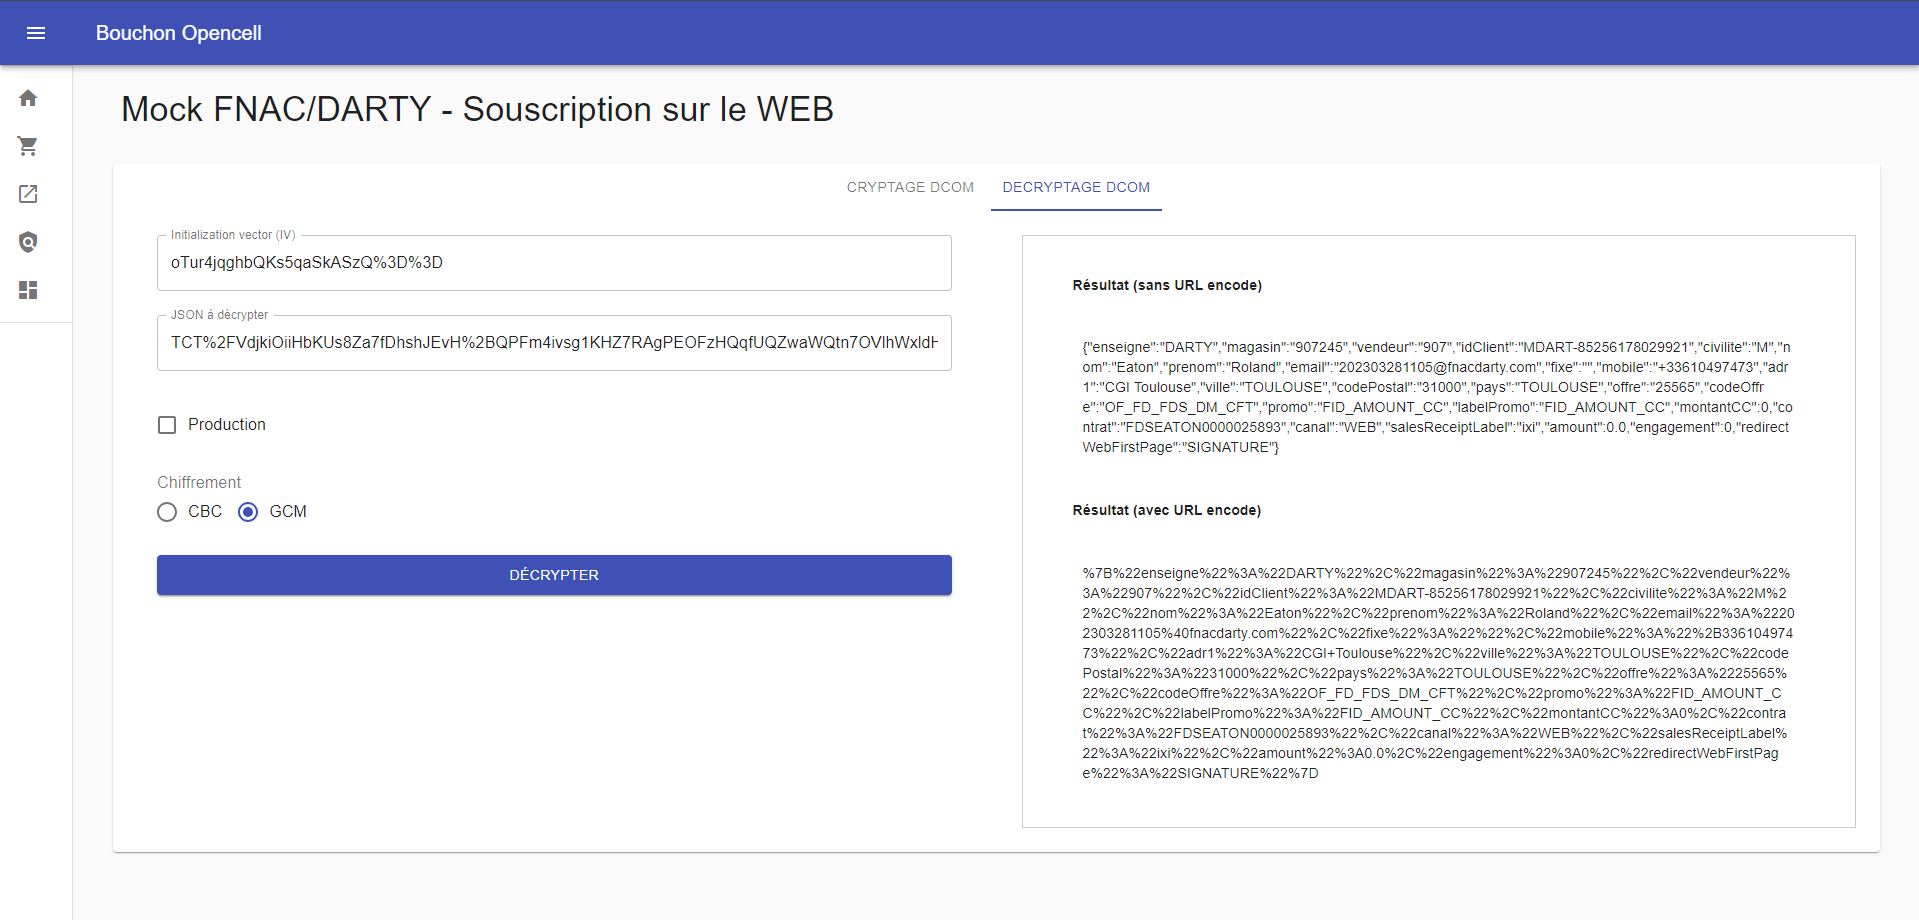
\includegraphics[width=1.45\textwidth]{assets/images/mock_before.png}
	\end{figure}

	\newpage
	\section{Le décryptage d'URL après la mise à jour du Mock}
	\label{sec:mock_after}
	\begin{figure}[!h]
		\centering
		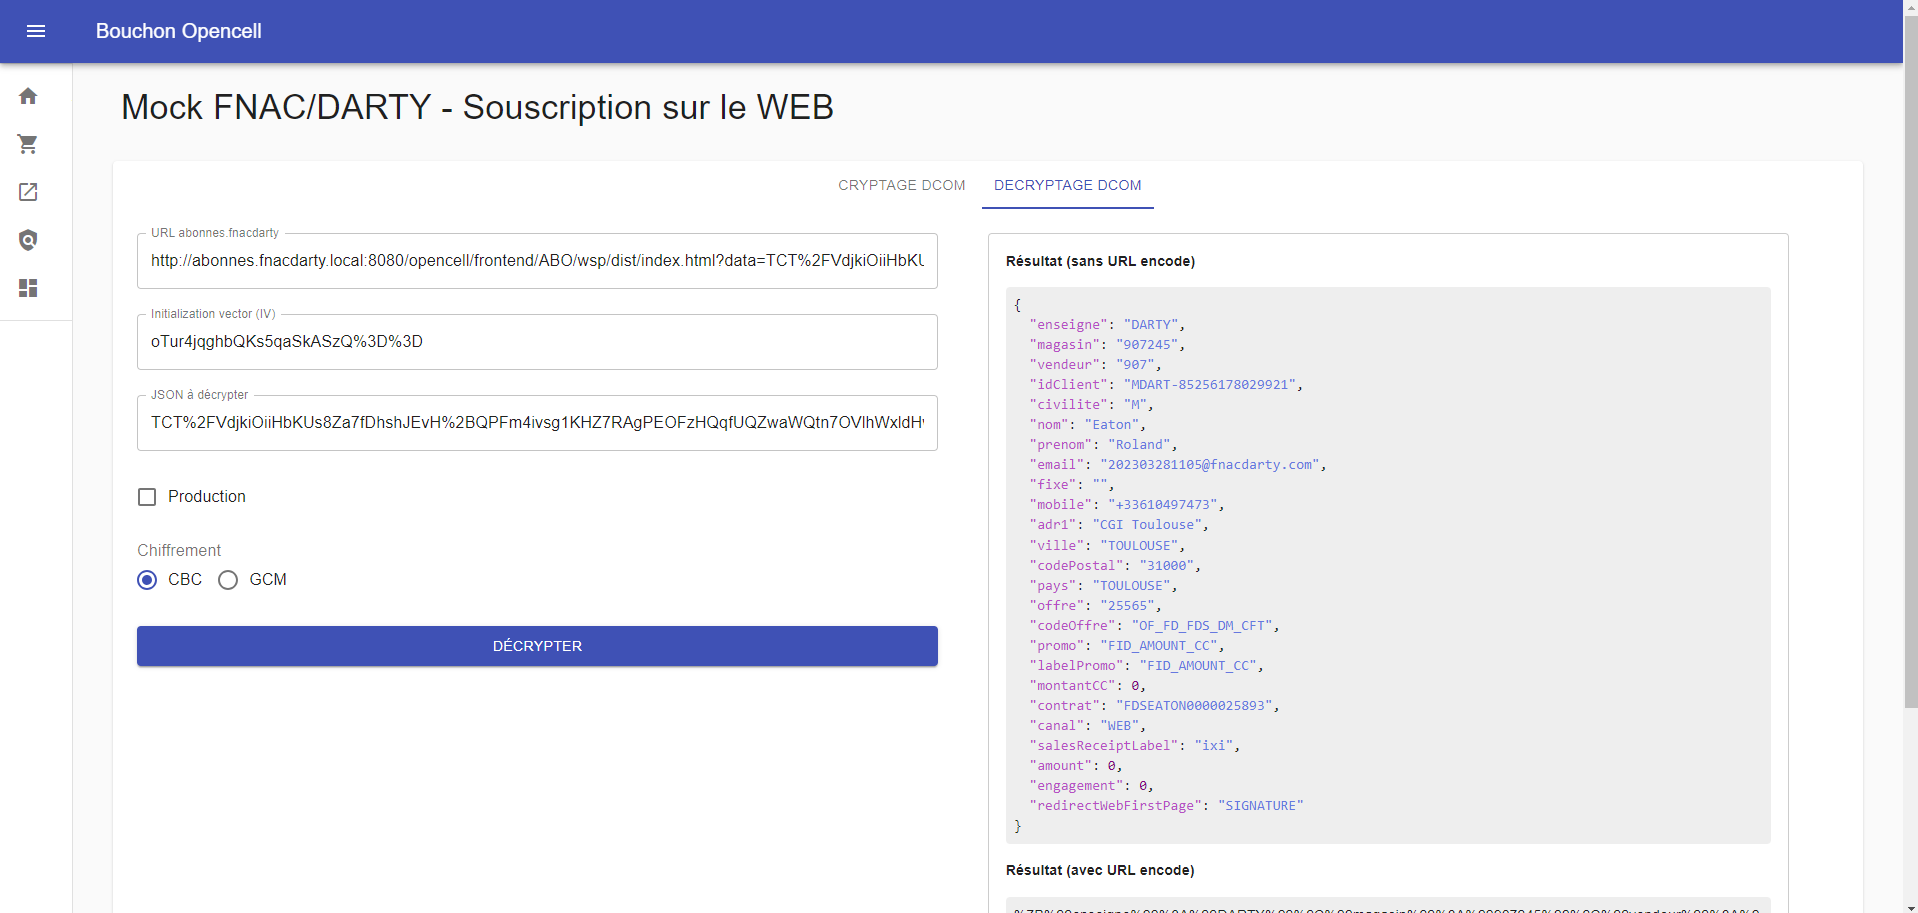
\includegraphics[width=1.45\textwidth]{assets/images/mock_after.png}
	\end{figure}

	\end{landscape}

	\section{CI/CD GitLab pour les applications front-end}
	\label{sec:ci-cd_gitlab}
	
\begin{minted}[bgcolor=cverbbg, breaklines, linenos]
{yaml}
default:
  # Default docker image for all jobs
  image: node:18-alpine
  tags:
    - darty

# Les étapes commentées ne sont pas présentes dans cette annexe
# Pour ne montrer que les parties pertinentes éditées lors du stage
stages:
  - lint
  # - build-deps
  - build
  # - test
  # - package
  # - docker-build
  # - deploy

.build-apps: &build-apps |
  function build_apps() {
    if [ "$1" = "prod" ]; then
      buildPath="prod"
    else
      buildPath="apps"
    fi;

    cd $CI_PROJECT_DIR/frontend/

    if [ "$1" = "prod" ]; then
      nx run-many --skip-nx-cache --parallel=6 --target=build,build-nomad
    else
      nx run-many --skip-nx-cache --parallel=6 --target=build,build-nomad --node-env=development
    fi;

    # copy each build into "build/*"
    for dir in $BUILD_DIRS
    do
      mkdir -p build/$dir
      if [ ! -d "dist/$buildPath/$dir" ]; then
        echo "Error: "dist/$buildPath/$dir" not found, compilation failed."
        exit 1
      fi

      cp -r dist/$buildPath/$dir/* build/$dir/
    done
  }
\end{minted}
\newpage
\begin{minted}[bgcolor=cverbbg, breaklines, linenos, firstnumber=46]
{yaml}
.lint-modified-files: &lint-modified-files |
  function lint_modified_files() {
    # Fetch SHA of the first and last commit of the diff between the target and source branches
    sha1=$(git log origin/$TARGET_BRANCH_NAME..origin/$SOURCE_BRANCH_NAME --pretty=format:%H --reverse | head -n 1)

    sha2=$(git log origin/$TARGET_BRANCH_NAME..origin/$SOURCE_BRANCH_NAME --pretty=format:%H | head -n 1)

    if [ "$sha1" = "$sha2" ]; then
      # If sha1 and sha2 are equal, set sha1 to the previous sha
      echo ">> Only one commit in the diff, getting the previous commit SHA1 to compare with the current one."
      logs=$(git log --pretty=format:%H $sha1^)
      sha1=$(echo "$logs" | head -n 1)
      echo ">> New $sha1 $sha2"
    fi

    # Get the list of modified files between the two commits
    diff=$(git diff --name-only --diff-filter=ACMRT $sha1 $sha2)

    filtered=""
    echo ">> Filtering files..."
    if ! filtered=$(echo "$diff" | { grep -E '^frontend.*\.(jsx|tsx|ts|js|mjs|cjs)$' || echo ""; }); then
      echo ">> Error occurred while filtering files."
      exit 1
    fi

    if [ -z "$filtered" ]; then
      echo ">> No files matched the pattern."
      exit 0
    fi

    # Get the list of files to lint
    files=$(echo "$filtered" | tr '\n' ' ')

    if [ -z "$files" ]; then
      echo ">> No files to lint"
      exit 0
    else
      echo ">> Files to lint:"
      echo $files
    fi

    npx eslint --max-warnings=0 $files
  }
\end{minted}
\newpage
\begin{minted}[bgcolor=cverbbg, breaklines, linenos, firstnumber=89]
{yaml}
lint-modified-files:
  cache:
    key:
      files:
        - frontend/package-lock.json
    paths:
      - frontend/.npm/
  stage: lint
  before_script:
    - apk add --update git
    - git fetch origin $TARGET_BRANCH_NAME
    - git fetch origin $SOURCE_BRANCH_NAME
    - cd $CI_PROJECT_DIR/frontend/ && npm ci --cache .npm --prefer-offline
    - *lint-modified-files
  script:
    - lint_modified_files
  only:
    - merge_requests
  allow_failure: true

# Build apps
build-apps:
  variables:
    BUILD_DIRS: st wsp vad cc sc nst tiers tiers-nomad dashboard
  cache:
    key:
      files:
        - frontend/package-lock.json
    paths:
      - frontend/.npm/
  stage: build
  before_script:
    - cd $CI_PROJECT_DIR/frontend/ && npm ci --cache .npm --prefer-offline
    - apk add --update git
    - *build-apps
  script:
    - \[ -z "${CI_COMMIT_TAG}" ] && build_apps "dev" || build_apps "prod"
  artifacts:
    paths:
      - frontend/build
  only:
    - triggers
    - merge_requests
    - web
    - tags
    - develop
    - /^release\/.*$/
    - master
\end{minted}

\makeutbmbackcover{}
\end{document}
